\part*{Project Description}
\chapter{Introduction}\label{ch:intro} 
% Needs to be less fluffy.

Ever since the inception of the modern internet, the information giants, such as
Google, Yahoo and Amazon, have been aiming for more and more personalisation in
their web-services, as the more personally relevant information and products are
to the user, the more likely they are to engage with it
\citep[p.8]{pariser2011filter}. Over the years, this constant aim to design for
personalisation has led to a situation, where web-services are always trying to
present users with the information which is most likely to cause a positive
reaction, while hiding information which could cause a negative reaction
\citep{filterBubbleDef, Personality}. This highlighting and hiding of
information is what activist and author Eli Pariser has coined the term ``The
Filter Bubble'' \citep[p.9]{pariser2011filter}. He describes the filter bubble
as an invisible filter which users can easily fail to notice, as it is not
something that you actively choose to engage with. This is fundamentally
different from old-school media, as the user would expect a certain filter or
viewpoint whenever they turned on a specific news station or news website
\citep[p.10]{pariser2011filter}. While this problem appears to be centred
around the large information giants, Pariser mentions that the problem also
persists on social media like Facebook, where content recommendations are
becoming increasingly personalised to the point where he experienced that
Facebook was no longer showing him content opposing his political views
\citep{pariserTedSummary}. While users might think that the people they surround
themselves with should represent many varied world views, the average person's
Facebook friends will be more likely to have the same opinions and share
information from the same news sources \citep[p.66]{pariser2011filter}.\nl

If we accept Pariser's idea of the filter bubble and consider that, as of August
2017, upwards of 67\% of adults in the United States report that they use social
media as a source of information \citep{journalism2017}, we can see a
situation where users are likely to only receive information confirming their
existing viewpoints and beliefs. The existence of this filter
bubble results in the problems which are tackled during this project, namely
how to assist internet users in identifying their filter bubble and giving them
the necessary tools to break it.

% The internet is widely used to find and gather information about any topics, it
% provides a vast amount of information from many different sources, and it is
% only growing larger. While easy access to information is a definite benefit, the
% enormous amount of information results in each user acquiring a small subset of
% the available knowledge.\\
% 
% Theoretically, this would not be a problem, as users could use the dynamics
% reach of social media to engage with information and news from different
% sources. But in reality, users tend to surround themselves with like-minded
% people, who in turn are prone to share information that correlates with their
% own opinions and biases.\\
% 
% This phenomenon is known as the ``Filter Bubble", which is a term coined by Eli
% Pariser in his 2007 book ``The Filter Bubble" \citep{pariser2011filter}.
% This Bubble refers to the effect of either selectively choosing information
% sources based on personal bias or actual algorithms encoded in the social media
% sites or search engines.
% The aim of which is to present the user with the information which is most
% likely to be regarded positively.
% The existence and enforcement of this bubble can cause problems, in which users
% avoid getting their opinions challenged by preventing them from being exposed to
% information and views that are opposed to the bubble in which they find
% themselves 
% %\citep[p.59-73]{pariser2011filter}\fix{}{So many pages?}.\nl
% 
%  In an interview with Eli Pariser, a
% search on ``Egypt'' shows a case of Google filtering information based on the
% user's preferences. In this example, two users would make a Google search with
% the term ``Egypt'', and end up with two widely different set of results.
% One user got results with information about ongoing conflicts and news; the
% other user saw travel guides and hotel booking information \citep{nusSduSearch}.
\subsection*{Initiating Problem}


Based on this, we can formulate the following initiating problem:


\begin{center}
\begin{minipage}{0.8\linewidth}

\textit{How can a filter bubble be identified by using social media and a web
agent?}

%\textit{How can an interner user search for a topic and find information from
%outside their filter bubble and how are social media sites used to create a
%filter bubble?
%How can a web agent be developed to identify the user's
%filter bubble from web activity and provide results from outside that bubble?}

\end{minipage}
\end{center}



\part{Analysis}

\chapter{Data Gathering}\label{cha:DG}
%Klaus: it would be nice to provide an overview to this chapter either here or
% on analisis part (Har smidt den efter initerende problem)
\chapter{Data Gathering}\label{cha:DG}
In order to identify a user's filter bubble, we need to analyse that user's
online activity, such that we can determine what people and information they
engage with. A user's online activity consists of large amounts of information,
including data on what websites they frequent, or which people they engage with
on social media. In the case of social media, this activity data get stored on
that site's servers, and in the case of browsing history, the data can be stored
locally on the user's device. While the user's data contain a lot of both useful
and irrelevant information, the vast amount of user data requires extensive
analysis to deduce something about a user.\nl

As we will need a reliable way to gather large amounts of data about a user,
this chapter will be used to analyse different sources of data, and methods of
gathering said data. In \autoref{sec:Social} we present a number of different
social media, and discuss what data we can gather from them, and what tools they
have available for accessing the data. In \autoref{subsec:crawler} we discuss an
alternative approach to gathering data, namely by using a web-crawler.
Finally, we conclude what approach is the most suitable for information
gathering.

\section{Social Media}\label{sec:Social}
In order to find a source of user data, this section will be used to analyze a
number of prominent social media sites. These sites can be seen in
\autoref{tab:priminentMedia} with their number of active
users \citep{SocialMediaStats, AdvertiseOnReddit}.

\begin{table}[H]\centering
\begin{tabular}{|l|l|}\hline
\textbf{Social Media} & \textbf{Active Users (Millions)}\\\hline
Facebook & 2061 \\\hline
YouTube & 1500 \\\hline
WhatsApp & 1300 \\\hline
Messenger & 1300 \\\hline
Twitter & 328\\\hline
Reddit &  250\\\hline
\end{tabular}
\caption{Social media sites and their number of active users}
\label{tab:priminentMedia}
\end{table}

Based on the number of active users, the most prominent social media sites are
Facebook followed by YouTube. However, while YouTube is a large social media
site, it is mainly used to upload and share videos. As this data is difficult to
analyze, we have chosen not to not inspect YouTube any further. In
addition, services focusing on direct messages between users, like Messenger and
WhatsApp are omitted, as this data is not publicly available. As such, the most
suitable social media sites to gather data from, are websites where many users
are openly interacting with each other, and where opinions and information get
exchanged through text posts and comments. Such sites include Facebook,
Twitter, and Reddit.\nl

\subsection{Facebook Analysis}\label{sec:facebook-analysis}
Facebooks is a social media site with more than one billion users, each
sharing posts and personal details, all of which are useful in the analysis and
detection of a person's \fbp. Facebook is used by both private citizens and
businesses in order to organize events, communicate and share ideas. 

\subsubsection{Using Facebook}
Facebook has two different entities that can interact with one another in
different ways \Source.

\begin{itemize}
  \item \textbf{User:} A user is a private citizen to share information. A core
  part of the user is ``feed'' which continuously shows new posts from users
  and pages. Users are able to connect with other users via ``friendships'',
  which allows the user to see some of the posts on their feed.
  \item \textbf{Page:} A page can be used to either organize an event, a
  discussion forum or as a profile for a company. Users can mark these pages as
  ``liked'' which can be used both to get updates from the page, as well as to
  show others, what they like
\end{itemize}

% \subsubsection{User}
% A user is a private citizen to share information. A core part of the user is
% ``feed'' which continuously shows new posts from users and pages. Users are able
% to connect with other users via ``friendships'', which allows the user to see
% some of the posts on their feed.
% 
% \subsubsection{Page}
% A page can be used to either organize an event, a discussion forum or as a
% profile for a company. Users can mark these pages as ``liked'' which can be
% used both to get updates from the page, as well as to show others, what they
% like

\subsubsection{Facebook API}
Facebook prohibits crawling/scraping of their site with a few exceptions such as
crawlers made by Google and Apple respectively
\citep{FacebookRobotsTxt}\fix{}{How can a normal non-crawler making reader see
this}.
To access data on their site, they have created the Facebook Graph \ac{API} as
part of their developer platform, which requires a registration of one's
application, along with an accompanying \ac{API} key used when performing
queries.
In addition to this requirement, there is also a strict requirement of consent
from the user of an application, which needs to specify all the different types
of data that the application wants to access
\citep{FacebookGraphApiAccessTokens} \fix{}{Cant seem to find where this strict
thing is defined in the text so\ldots.}\Source .\nl

An analysis of Facebook's Graph \ac{API} \citep{FacebookGraphApiDocumentation}
reveals that the platform previously allowed for more freedom when gathering
information about a user and their social circles. However, this is no longer
the case as of version 2.0 of the \ac{API}
\citep{FacebookChangesInGraphTwoPointOh}.

The current \ac{API} is limited to only listing those of the user's friends
that are using the same app and have given consent to let the app use their
details \citep{FacebookChangesInGraphTwoPointOh}. Access to the user's ``likes''
is limited to the interests listed on their profile, such as their favourite
movies and pages on Facebook, that they have marked as ``liked''
\citep{FacebookGraphApiUserEdges} \citep{FacebookGraphApiUserLikes}
\fix{}{Might be a bit hard for a reader to understand where you got that
from these two sources}.\nl

It is possible to access the user's posts and details regarding them,
including whether they were originally posted by the user or shared from
another poster. These shared posts can then be traced back one or more steps
depending on the privacy settings of each link in the ``share--chain'', but
only limited information can be gathered about the users on the chain
\citep{FacebookGraphApiUserFeed}\fix{}{Please explain to me, where you can
see that about the share--chain}.\nl

Based on this information, it is possible to use Facebook's \ac{API} to find
further connections between existing users of the system.
Knowledge of these users, based on what the system has found out via other
sources, can then be used to either confirm or update the system's knowledge of
these individuals.
\section{Reddit Analysis}\label{sec:reddit-analysis}
Reddit is a social news aggregation and discussion website with over 250 million
registered users \citep{AdvertiseOnReddit}. The site is split into
``subreddits'' wherein users can post entries as plain text, pictures and links to other websites. \nl

Entries are ranked by the users who can either ``upvote'' or ``downvote''. This
is the case for entries and comments. \citep{AboutReddit}\nl

Users can follow other users such that all activity from the followed users is
shown in a designated tab.

\subsection{Reddit API}\label{subsec:reddit-api}

Reddit has a \ac{REST} \ac{API} that provides access to a user's information,
posts and comments in subreddits, as well as moderation tools, that allow for
manipulation of these \citep{RedditApi}. Software that interacts with the
\ac{API} must follow certain rules. These include using OAuth2 to ensure that a
user has given consent and that all requests are seen as coming from that user,
and checking the rate-limiting headers returned with every server response and
making sure to uphold them.
Additionally, every client should provide a specially tailored \ttt{User-Agent}
\ac{HTTP} header field, following the template: \citep{RedditApiRules}\nl

\begin{center}
  \ttt{<platform>:<app ID>:<version string> (by /u/<reddit username>)}
\end{center}\nl
\begin{description}
  \item[\ttt{platform}] a descriptive name for the platform type on which the client is running.
  \item[\ttt{app ID}] a unique name for the client, which could be formed like a Java package namespace.
  \item[\ttt{version string}] identifies the version of the client uniquely
  within the given \ttt{app ID}.
  \item[\ttt{reddit username}] is the username of the creator of a client who
  should be contacted by the Reddit team in case of problems.
\end{description}\nl

Spoofing another client or a browser using the \ttt{User-Agent} \ac{HTTP} header field is strictly prohibited and
results in a ban if discovered. \citep{RedditApiRules}\nl
\subsection{Twitter Analysis}\label{sec:twitter-analysis}
Twitter is a global social media site with more than 328 million active users
\citep{SocialMediaStats}. Twitter's have two types of users, private citizens
and businesses. While businesses might use Twitter for announcements and
marketing, private citizens are more likely to use Twitter for general
communication and to discuss global and local events. In general, Twitter
defines itself as being used for the following purposes \citep{StartingTwitter}:

\begin{enumerate}    
  \item News and Politics.
  \item Sports.
  \item Pop Culture. 
  \item Influencers.
  \item Utility.
\end{enumerate} 

\begin{figure}[H] 
	\centering 
	
\includegraphics[width = 0.8\textwidth]{figures/DonDrumpf.png}
	\caption{Example of an ``influencers'' tweet from \@realDonaldTrump.}
	\label{fig:DrumpF}
\end{figure}

\subsubsection{Using Twitter}
A Twitter user can make use of the following elements \citep{StartingTwitter}
in order to make tweets and communicate with other users:

\begin{itemize}
  \item \textbf{Tweet:} A tweet is a message, which a user can post from their
  account. A tweet can contain 280 characters \citep{Tweet280} of text, links,
  pictures and similar media sources, and be seen by all other users. Users who
  ``follow'' an account will automatically receive its tweet on their Twitter
  feed \citep{StartingTwitter2}.
  \item \textbf{Follow:} A user can choose to follow other peoples accounts,
  then they will get a notification whenever that account makes a tweet or
  retweets an existing tweet.
  \item \textbf{Retweet:} Instead of making a tweet, a user can forward a tweet
  made by another account. A user can choose to either retweet a tweet as it is,
  or embed the tweet into a tweet of their own. A user can make comments or
  remarks concerning the original tweet \fix{}{The last part,
  does the source not say}.
  \item \textbf{Hashtag:} When a user tweets or retweets, they can add a
  ``hashtag'', which can be used to group the tweet, with other tweets
  containing the same hashtag. Examples of hashtags usage on Twitter could be
  \#Politics or \#Sports, or to specify the user's opinion on a subject, e.g.
  \#war \#Idiotic. On Twitter hashtags are used for grouping, searching and
  filtering \fix{}{Much more than the source say}.
\end{itemize}

% \subsubsection{Tweet}
% A tweet is a message, which a user can post from their account. A tweet can
% contain 280 characters \citep{StartingTwitter2} \fix{}{That is not someting
% that source says} of text, links, pictures and similar media sources, and be
% seen by all other users. Users who ``follow'' the account will automatically be
% presented with the tweet on their Twitter feed.
% 
% \subsubsection{Follow}
% A user can choose to follow other peoples accounts. Then they will get a
% notification whenever a followed account makes a tweet or retweets an existing
% tweet.
% 
% \subsubsection{Retweet}
% Instead of making a tweet, a user can choose to forward a tweet made by another
% account. A user can either retweet the tweet as it is, or embed the tweet into a
% tweet of their own. A user can make comments or remarks in relation to the
% original tweet \fix{}{The last part, does the source not say}.
% 
% \subsubsection{Hashtag}
% When a user tweets or retweets, they can add a ``hashtag'', which can be used to
% group the tweet, with other tweets using the same hashtag. A hashtag is used as
% a general tag, such as \#Politics or \#Sports, or to specify the user's
% opinion on a subject e.g. \#war \#Idiotic. In general, hashtags are used for
% grouping, searching and filtering  \fix{}{Much more than the source say}.

\subsubsection{Twitter \acp{API}} \label{sub:twitterapi}
Twitter permits developers to retrieve data from their users, tweets and
trending hashtags. Twitter has three main \acp{API}, namely the \ac{REST}
\ac{API}, the Streaming \ac{API} and the Ads \ac{API} \citep{TwitterDevDocs}.
For this project, the \ac{REST} \ac{API} is the best fit, as it permits reading
Twitter' user data.

\subsubsection{REST API}
The \ac{REST} \ac{API} makes use of \ac{HTTP} requests to allow developers
access to Twitter's data \citep{TwitterREST}. Also, by using the OAuth protocol
\citep{TwitterOAuth}, Twitter enforce that only authorised applications can
access Twitter's data. All requests must be made using the \ac{HTTP} protocol.
These requests are structured differently based on the requested data.
\autoref{httpReq} shows an example of a \ac{HTTP} request with each part denoted
with a number and further explained in \autoref{httpReq}.

\figx{httpReq}{Structure of Twitter HTTP Request.}

\begin{table}[H] 
\begin{centering}
\begin{tabular}{|l|p{9cm}|l|}
\hline
\textbf{No}&	\textbf{Description}										\\\hline
1			&	Denotes the type of request: GET, POST, DELETE.				\\\hline
2			&	Address for the Twitter \ac{API}.							\\\hline
3			&	Name of the requested resource.	   							\\\hline
4			&	Format of the requested resource.							\\\hline
5			&	Index of the page of the requested data. In case all data can not be
retrieved in a single page.													\\\hline 
6			&	Extra parameters such as the name of the requested user.	\\\hline
7			&	Number of data points requested. Maximum of 5000 per page.	\\\hline
\end{tabular}
\caption{Elaboration on the Twitter HTTP requests.}
\label{httpElaboration}
\end{centering}
\end{table}

\fix{}{Some kind of connection logical followup to Web Crawler}

In this chapter, it will be investigated what a Web Crawler is including, how it
is created, how it works, what it can gather and its limits. in the end, we will
conclude upon if a crawler is a suitable substitute or supplement to
the Twitter \ac{REST} \ac{API}.

\subsection{Web Crawler}\label{subsec:crawler}
A crawler, which is also known as a spider, systematically crawls the internet
and gathers information by reading and analyzing the content of web-pages.
Web-pages are usually connected to each other by hyperlinks, which a
crawler can use to move between pages. This recursive approach to accessing
web-pages allows the crawler to systematically access large parts of the
internet, and gather data along its journey. %'Recursive approach'

\subsection{Crawler design}%Fluffy start på section 
There are several things to consider during the crawlers execution. A crawler
must be able to avoid getting stuck fetching an infinite number of pages from
the same domain, as this is only acceptable if you want to crawl that specific
site.
The crawler needs to be ''polite'' about how frequent it makes requests to a
server, as too many requests to the same server can crash it, or cause the
server to consider the crawler an attacker and block it.
The crawler should respect what it is, and is not, permitted to access from a
given domain. Additionally, the crawler should also be able to re-fetch data
from older sites, in order to see if they have been updated. Additionally, it
should favour fetching pages that are more likely to have quality content \citep[Ch.
20.1]{manning2008introduction}.\nl

Generally, a crawler's architecture is made to be modular, which can be seen in
\autoref{BasicWC}. The 'Frontier' is a list of elements, usually URLs, which
have not been crawled yet. The 'Fetch' module is designed to get the first
element from the 'Frontier' and request access to the corresponding site. The
site content is passed to the 'Parse' module, which is further described in
\autoref{sec:parsing}. The site content gets verified to find if the site has
been crawled before, it could be that the side had minor updates or called
itsef recursively causing the crawler to loop.
The URLs are filtered according to the domains ``/robots.txt'', which describes
what each crawler is allowed to access. Finally, the duplicate URLs are
eliminated, and the new URLs are added to the frontier.\nl%Sjov formullering?


%Vejleder vil gerne have fikset overfull boxes men det er på den måde i bogen.
\figx[1.2]{BasicWC}{The basic crawler architecture \citep[p.
446]{manning2008introduction}.}
%Klaus: Some more sentances of explanation. It is always good to give the reader
% some basic understanding of what is going on in the caption, even if it
% doubles a bit with normal text

% Flesh out more
A more advanced version of a crawler involves managing multiple, distributed
crawlers. These crawlers need to work together to cover websites faster and
avoid crawling the same sites multiple times, they should also avoid spamming
the same servers with requests.


\subsection{Parsing} \label{sec:parsing}
Parsing is a method used to extract information from a document, and index it
for later use. In this case, a document is the raw-content retrieved from a request,
including text, HTML code and -tags.
The first part of parsing a document consists of removing the unnecessary
information, such as HTML tags, while retaining the important information, like
links and the body text. Depending on the document, it may be necessary to
decode the document format and its character encodings.
The second step is to tokenize the text, which means splitting up the text into
the smallest meaningful entities, which in this context are words. Depending on
how advanced the tokenizer is, it should be able to handle abbreviations, such
as ``aren't'' or ``kg.''. The tokenizer should also remove stopwords, which are
words that do not contain useful information, and should therefore not
be indexed. Examples of this are words such as ``the'' and ``a''. As these words
do not refer to anything in particular, a query should not match indexed pages
based on them \citep[Ch. 2]{manning2008introduction}.

\subsection{Indexing}
Indexing is used to speed up the information retrieval process, as it is faster
to search an index than to scan through every single page every time a query is
performed.

There are different types of indexes, the best fit depends on the way
that the tokens and documents refer to each other. The two main types are the
forward index and inverted index, examples of such can be seen below.

\begin{minipage}{.40\textwidth}
  \centering
  \begin{table}[H]
	\centering
    \begin{tabular}{|l|l|}
\hline
Doc1 & fresh, tomato, soup \\ \hline
Doc2 & fresh, potato, soup \\ \hline
Doc3 & fresh, tomato, sauce \\ \hline
	\end{tabular}
	\caption{A forward index.}
	\label{fIndex}
  \end{table}
\end{minipage}
\begin{minipage}{0.5\textwidth}
  \centering
  \begin{table}[H]
	\centering
    \begin{tabular}{|l|l|}
\hline
fresh & Doc1, Doc2, Doc3 \\ \hline
tomato & Doc1, Doc3 \\ \hline
soup & Doc1, Doc2 \\ \hline
sauce & Doc3 \\ \hline
	\end{tabular}
	\caption{A simple inverted index.}
	\label{iIndex}
  \end{table}
\end{minipage}\nl

In a forward-index the pages themselves are indexed with a reference to the
tokens they contain, see \autoref{fIndex}. An inverted-index is made up of
tokens referencing the documents containing them, this is useful when
querying for specific tokens \citep{Index3}, see \autoref{iIndex}. More advanced
indexes can be expanded to include ranking of the tokens to better
evaluate a documents information value. This ranking is usually determined by
how often the token appears in the crawled documents, and how many times it
appears in a specific document.

\subsection{Data Gathering Conclusion}

%Skal vi lige have en kort afslutning om hvad vi lærte og hvorfor vi bruge API?


%What did we learn in this chapter? a conclusion would be nice. I realize that
% one exists in the next section, but you cango into greater detail here.

\section{Social Media Conclusion}\label{sec:social-media-conclusion}
After considering the three sites Facebook, Reddit and Twitter, and
analysing the possibilities they provide.\nl


The decision was based on ease of use, level of access, and the short form of
tweets from Twitter. It is expected to provide more results of a smaller size
resulting in less data to analyse overall. Twitter is also less locked down with
a public default setting, making it easier to access enough information to
identify a \fb. It is expected that the because the tweets are short then they
will be more direct, because Twitter enforces a strict 140 character limit on each
tweet. Therefore, it is expected that sifting through the data will require less
effort.\nl

What are the methods most commonly used to gather information from multiple web
pages, and can it be done in a way to permitting easy search through data from
multiple social media sites?

\chapter{Data Analysis}\label{cha:DA}
\chapter{Data Analysis}\label{cha:DA}
In order to make use of the tweet data from Twitter, it needs to be analyzed in
order to extract the useful elements. One of these methods is known as a sentiment
analysis, which attempts to determine the opinions of people regarding specific
topics, such as movies or products. This technique has become especially useful
for social media, as people increasingly discuss and post their opinions online
\citep[Overview 2]{Sentiment}. Additionally, since sentiment analysis can be
used to determine users opinions on products, it should be possible to apply
this analysis on politicians, legislature, political events, and other political
keywords.\nl

Sentiment analysis is done by gathering text post
and comments, and extracting features providing clues to the opinion. The
features can then be used with a classification model to predict the
sentiment.\nl

In \autoref{sec:FeatEx} we examine how to transform text into useful
\textit{features}, and which options are available to increase the quality of
those \textit{features}. In \autoref{sec:Class} we will look at how the
\textit{features} can be used in models to make predictions. In
\autoref{sec:mediaAnalysis} we discuss how user's preference in news media can
help in indicating their political leanings. Finally in \autoref{sec:DAConc} we
will conclude on the analysis.

\section{Feature Extraction}\label{sec:FeatEx}
Feature extraction is a method used after the tokenization, to choose which
words best determine the sentiment. Much can be lost in the feature extractor,
as the opinions are more apparent in text than as a series of tokens. There are
several ways to express the sentiment in a text, such
as\citep[Overview.3-4]{Sentiment}:


\begin{itemize}
  \item Capitalization. 
  \item Lengthening.
  \item Punctuation.
  \item Stopwords.
  \item Negation.
\end{itemize}

For instance, there is a big difference between person one saying ``I love this
movie'' and person two saying ``I LOVE this movie!!!!''. In this example, both
the capitalisation of ``love'' and the exclamation mark helps to emphasise that
person two seems to have a stronger positive sentiment towards the movie.\nl

An example of lengthening as a difference in sentiment could be between
``huuuungry'', ``huuungry'' and ``hungry". The differences in sentiment between
the first two variations of ``hungry" are probably minimal, but there is an
apparent difference between those and the last version. To compress these
features one can look for tokens with more than two of the same letters repeated
and removing the repeated letters. This will make the loss of sentiment minimal
while limiting the variations of the same word.\nl

It is useful to remove stopwords, which are words that do not contain valuable
information. As they can appear in every type of sentence, they can make
classification more difficult, though it also mainly depends on the model,
see \autoref{subsub:Models}.\nl

Negation also needs to be considered, as the sentiment can be changed entirely
with a word ``not''. Because sentiment gets extracted from tokens, it is
difficult to judge how each token relate to others when seen individually. A way
to handle negation is to prefix tokens with a tag such as ``NEG\_'' after a word
like ``not'' and ``aren't''.\nl

See \autoref{tab:feature} for an example of how a feature extraction can look.

\begin{table}[H]
\centering
\begin{tabular}{|p{6cm}|p{8cm}|}
\hline
Text & Features \\ \hline
I LOVED the movie but I am sooooo hungry! & 
``I'' ``LOVED'' ``movie'' ``I'' ``soo'' ``hungry'' ``!''
\\ \hline 
I don't like this song, why do they keep playing it? &
``I'' ``dont'' ``like'' ``NEG\_song'' ``NEG\_why'' ``NEG\_keep'' ``NEG\_playing''
``?'' \\ \hline
\end{tabular}
\caption{An example of transforming text into features.}
\label{tab:feature}
\end{table}

There are a couple of other methods that can affect how much sentiment is
retained in the text, such as stemming and using n-grams.

\subsection{Stemming}\label{subsec:Stem}
Stemming is a method used with feature extraction, to collapse a word into its
base, for instance ``finding'' can be stemmed to ``find''. Stemming is both
useful and destructive. It allows for a reduction in the number of terms by
collapsing them. It is also destructive as sentiment clues can get erased. The
meaning of a word can often have ties to the ending of the word, such as
``captivating'' and ``captive''. By using the Porter Stemmer Algorithm, both
words will collapse to ``captiv'' which removes what differentiate them. There
are other Stemmer algorithms, but each provides similar problems. Stemming can
be useful as it can reduce the vocabulary, instead of remembering both
``captivating'' and ``captive'', it now only needs to remember ``captiv''. This
can be useful for small datasets where each token is important, as it can reduce
the vocabulary size and sharpen the result \citep[Ch 3.b]{Sentiment}.

\subsection{N-Grams}
N-grams are a sequence of 'n' items and determines how much context is stored
from a piece of text. An example of the three first n-grams, seen in
table \autoref{tab:ngram}.

\begin{table}[H]
\centering
\begin{tabular}{|l|l|}
\hline
Text & ``I love horror movies'' \\ \hline
Unigrams (1) &
``I'' ``love'' ``horror'' ``movies''
\\ \hline 
Bigram (2) &
``I love'' ``love horror'' ``horror movies''
\\ \hline
Trigram (3) &
``I love horror'' ``love horror movies''
\\ \hline
\end{tabular}
\caption{An example of different N-Grams}
\label{tab:ngram}
\end{table}

The idea is that as bigger n-grams are used, more context gets stored in the
token. It becomes less likely to encounter a given token, which should
improve accuracy if there is a large training sample. With smaller training
samples it becomes necessary to use unigrams as there are not enough
token occurrences to justify using bigger n-grams.

\subsection{Feature Vectors}\label{sub:FeatureVector}
A feature vector is used to denote which features are present in a piece of
text. The vector gets created by mapping each feature to a unique integer, this
is done while training the model and is called a Bag-Of-Words (not to be
confused with the Bag-Of-Words classification model, described in
\autoref{subsub:Models}). With this Tokens-To-Integers the feature vector can
now be created as a series, often array, of 1's or 0's, which denotes whether
the given feature is present in the vector. The bigger the Bag-Of-Words is, the
larger every feature vector is. For example if ``\textit{love}'' is mapped to
\textbf{3} and ``\textit{movie}'' is mapped to \textbf{205}, then a feature
vector for ``\textit{I love this movie}'' could be: [0,0,0,1,0,\ldots,0,1,0].


\section{Classification}\label{sec:Class}
The final part of a sentiment analysis is the classification task. This task
consists of predicting the sentiment based on the features extracted earlier.
The accuracy of the predictions is based on the labelled data provided as
training data, as well as the model used.

\subsection{Training}\label{subsec:Train}
The training data is an important part of every model. There are three
different training methods, each suitable for a different task.

\begin{itemize}
  \item \textbf{Supervised learning} is when the training data is paired as an
  input-output pair, for instance: ``This is a great movie'' can be paired with
  ``positive''. This pairing allows the model to verify its prediction whether
  it guesses correct or not \citep[Ch. 7.0]{MIBook}. This method is useful as it
  provides an easy way to validate the accuracy of the model. The main problem
  is that most data is not labelled, which means that it has to be labelled for
  it to be useful.
  \item \textbf{Reinforcement learning} is similar to supervised learning with
  the key difference being that the model is only given a ``reward'' when it
  performs the best action. This type of learning method is useful when training
  a robotic agent \citep{Reinforcement}.
  \item \textbf{Unsupervised learning} is different as the training data no
  longer includes a result, and as such, it can no longer evaluate the accuracy
  of the prediction. Instead, it allows for clustering data and aims to minimize
  prediction errors \citep[Ch. 11.1]{MIBook}.
\end{itemize}

The most used model for sentiment analysis, is the supervised learning approach,
as it is the most useful for classification tasks.

\subsection{Models}\label{subsub:Models}
There are several different models used for sentiment analysis. Different models
provide varying levels of accuracy, as seen in \autoref{sentiment}, which shows
several different models on the same IMDB dataset, with three different outputs.
While we do not go in depth about all the models that are available, we will
describe the models that are of immediate interest to us. A cursory description
of different models can be found in the citation \citep{Classification}.

\figx[1.0]{sentiment}{Accuracy of different sentiment analysis models on the
IMDB dataset \citep{Classification}.}

Our main focus will be on the Bag-Of-Words and Naive Bayes models, as both
are straightforward methods of determining sentiment, which should help with
providing proof of concept.

\subsubsection{Bag-Of-Words}
The Bag-Of-Words model determines the sentiment of a text by counting the
occurrences of words with either a negative or positive attitude. Some models
simply count the occurrences of positive or negative words, but int other models
words can have different sentiment scores where one word may be perceived as
conveying a more intense sentiment than others. Each word and its corresponding
sentiment score gets stored in a sentiment lexicon, these lexicons can be
created by or found freely online \citep{BagOfWords}. An example of words and
their sentimental value can be seen in \autoref{tab:bowwords}.

\begin{table}[H]\centering
\begin{tabular}{|l|l|}\hline
\textbf{Word:} & \textbf{Sentiment:} \\\hline
LOVE	&	15	\\\hline
Love	&	10	\\\hline
Like	&	5	\\\hline
HATE	&	-15	\\\hline
Hate	&	-10	\\\hline
Dislike	&	-5	\\\hline
\end{tabular}
\caption{Sentimental words and their corresponding values}
\label{tab:bowwords}
\end{table}

\subsubsection{Naive Bayes} 
The Naive Bayes classifier uses Bayes' rule and the assumption of independence,
which simply assumes that the features are independent of each other
\citep[Proposition 6.5]{MIBook}, to determine the sentiment. Bayes' rule, see
\autoref{e:Bayes}, describes how prior knowledge can relate to and affect an
event \citep[P.229]{MIBook}. 

\begin{equation}\label{e:Bayes}
P(X|Y) = \cfrac{P(Y|X) \cdot P(X)}{P(Y)}
\end{equation}


It trains using supervised learning, where each text object gets labelled with a
class. The text features get extracted as tokens and, the probability of each
token belonging to each of the labels is then calculated, by counting how often
it occurs with each class; leading to a table such as \autoref{tab:NB}.

\begin{table}[H]
\centering
\begin{tabular}{|l|l|l|l|}
\hline
Word & Positive & Negative & Total 	\\ \hline
this & 45 & 55 & 100				\\ \hline
movie & 115 & 85 & 200				\\ \hline
rule & 90 & 10 & 100				\\ \hline
suck & 5 & 95 & 100					\\ \hline
Total & 255 & 245 & 500				\\ \hline
\end{tabular}
\caption{A table where each token is classified with a label.}
\label{tab:NB}
\end{table}

To predict which class, \textit{C}, a given piece of text belongs to it needs to
be transformed into a feature vector, \textit{W}, where each feature gets
denoted as, $w_{i}$. By using \autoref{e:Score} we can predict the class
\citep[Ch.2.1]{Bayes}.
\begin{equation}\label{e:Score} score(W,C) = P(C) \cdot
\displaystyle\prod_{i=1}^{n}P(w_{i}|C)
\end{equation}

The idea is to calculate the probability of the feature vector belonging to each
of the classes. The class probabilities $P(C)$ are determined how frequently the
classes have been observed to occur, therefor:
\begin{center}
$P(C_{Pos}) = \cfrac{255}{500} = 0.51 $ and $P(C_{neg}) = \cfrac{245}{500} =
0.49 $
\end{center}
The probabilities of each of the features are likewise found by how often the
features occur. For instance, if we want to determine the class of ``this
movie rule'', with the probabilities from \autoref{tab:NB}, we get the
following feature vector [1,1,1,0]. We can then calculate the score of
the feature vector belonging to each of the classes:

\begin{equation}\label{e:Pos}
score(W, C_{Pos}) = \cfrac{255}{500} \cdot \cfrac{45}{100} \cdot
\cfrac{115}{200} \cdot \cfrac{90}{100} = 0.238
\end{equation}
\begin{equation}\label{e:Neg}
score(W, C_{Neg}) = \cfrac{245}{500} \cdot \cfrac{55}{100} \cdot \cfrac{85}{200}
\cdot \cfrac{10}{100} = 0.019
\end{equation}

Then by taking the highest score we the can predict the class the text belongs
to, in this case, it would be positive.

\section{Media Analysis}\label{sec:mediaAnalysis}
When retrieving tweets from Twitter we can also recieve some additional
information such as location, timestamps, and shared links. Among these, shared
links specifically can be used to determine a user's political leanings. This is
based on the fact, that news media sites often have an inherent political bias
\citep{allSidesMedia}.

\section{Data Analysis Conclusion}\label{sec:DAConc}
After considering how sentiment analysis is used to analyse data, we can
conclude that it has distinct uses for classifying vast amounts of user data. It
is especially useful for analysing the sentiment around American politics as
there are only two main parties with opposing views, which means that not only
are there few classes, they should also be very distinct. By determining the
sentiment, it becomes possible to see if a user is inside a political bubble,
where the user only encounters the same sentiment.



%https://www.cs.cornell.edu/home/llee/papers/sentiment.pdf



\chapter{Problem Statement}

Throughout the analysis, we have investigated how to identify and break out of a
filter bubble. As such, this section will be used summarize the conclusions, and
define a problem statement.\nl
%Klaus: I'm not sure I agree with this statement. I believe you rather compared
% social media sources and then a bit about data gathering

In \autoref{cha:SocialMediaAnalysis} we came to the conclusion, that Twitter is
most suitable for gathering data, as it provides an \ac{API} that allows us to
easily request all relevant data for a user. This data can be requested from any
user, who has not set their account to private. The data consists of tweets,
followers, and friends for any such user.\nl

In \autoref{cha:DataGathering} we discovered that there are restrictions to what
a crawler is allowed to access. We have determined that while it is possible to
use a regular crawler to gather data, it is preferable to use the official
Twitter \ac{API} designed for the purpose. We made this decision, as the
\ac{API} gives access to all relevant data by using a simple set of \ac{HTTP}
requests, while a crawler has to adhere to a stricter set of limitations.
However, we are still able to use the crawler architecture as a guideline for
how to design a solution.\nl




% In \autoref{emotions} we determined that we can identify a users filter bubble
% by how ``emotional'' they were about certain topics. This can be done by
% pairing key topical words like names of political figures, with emotional
% words like ``like", ``good", and ``hate".\nl

Based on these conclusions, we can establish the following problem statements:

\begin{center}
\begin{minipage}{0.95\linewidth} 

\textbk{How can a software solution be developed as to permit a user to break
out of a filter bubble by using information gathered from social media. And how
can the developed software allow identify a user's filter bubble, and present
the user with information from outside of it?.}

\end{minipage}
\end{center}





%\chapter{Initial Ideas}
By researching how to break the filter bubble, we have identified two potential
solutions. These sulutions aim to break the filter bubble by analyzing what
information the user is presented with, and categorizing it based on the media
source, and the words the users friends use to describe this information.\nl

In general, both solutions will make use of a neural network in order to
categorize tweets and determine the filter bubble.

\section{Analyze News Media}
The first solution is to analyze tweets and retweets in order to identify all
news articles, and what news media they originate from. These news media would
be classified based on their political bias, and this information will be use to
determine the filter bubble for the given user.\nl

The benefit of this solution is that it should be easy to determine a users
source of news information, and that information already exists about news
sources politiacal biases. In addition, if we can identify a political bias
amound the tweets a user is presented with, it should be possible to break the
filter bubble by presenting information from another point on the political
spectrum.

\section{Analyze Words}
Another solution is to analyze the content of each individual tweet, and
determine any nouns and the adjectives used to describe them. Based on the
positive/negative connotation of these words, we can determine what people think
about a given subject.\nl

The benefit of this solution would be, that it is not limited to using news
sources, but instead can be used on all nouns present in tweets. As such, it can
be used to determine a users filter bubble on any given subject. The problem
with this solution is that it would be difficult to break the filter bubble, as
we cannot easily determine what information to present the user.

\section{Combined Solution}
Another solution would be a combination of the prior two, where we attempt to
determine the bias of a users news sources, and attempt to strengthen our model
by analyzing what users think of the presented news articles. This would
strengthen our model, as we would be able to identify if a retweeted article is
based in a users support or dislike of said article.
 Fluffy needs to be written

\chapter{Requirements Analysis?}
\chapter{Requirements Definition}\label{cha:req}
Following the problem statement in \autoref{ch:problem}, this chapter will be
used to determine the actual requirements of the developed software solution.

% Klaus: The web aspect seems to be missing? From the study regulations: A
% suitable user interface implies that it is possible to interact with the
% developed solution using a web based interface.
% E.G., an end user application has a web based user interface. An agent or a
% service may not necessarily have a web based user interface, but would usually
% have a web based A further reuirement is that the implementation needs to have
% ascalaable acrhitecture

\section{Functional Requirements}

\begin{requirement}[req:twitter-user-retrieval]{Retrieve user and pertinent information from Twitter}
Given a Twitter username, the program should be capable of retrieving
tweets and information about a user, including the accounts they are following.
\end{requirement}

\begin{requirement}{Follow Twitter \ac{API} guideline} 
The program should follow the Twitter \ac{API} guidelines such as not making
more requests than the guidelines specifies per. 15 minutes. This guideline
means that the program should also be capable of keeping track of how many
requests it has used, how many it is allowed to use and when the limit resets. 
\end{requirement}

\begin{requirement}{Identify political beliefs of a user}
The program should be able to identify and inform the user of his or her
political belief and of that of those he or she follows. It should do this by
analysing the words, hashtags and links.

% Saved for a little while 12-12-17
% Using the links and comparing them to the list of bias news site and also taking
% into account the emotional words, the program should be able to identify and
% inform the user of his/her political beliefs. 
% The program should be able to identify hashtags and \acp{URL} in the downloaded
% tweets such that they can be used for bias analysis of the user who posted it or
% the user following the user that posted it.
% The program should be able to use the links identified in the tweets and compare
% them to a list of bias news site which should be created and stored in the
% program. 
% The program should be able to identify and use emotional words to examine a
% users view on different subjects in the tweets.
\end{requirement}

\begin{requirement}{Web-Application Front-End}
The application should make use of a front-end developed as a web application.
This application should be hostable on a server such that it can be presented as
a web page.
\end{requirement}

\begin{requirement}{Server Back-end}
The logic of the developed software should be hosted on a server, which receives
requests from the front-end, and returns analysed data and the determined
conclusions.
\end{requirement}

\begin{requirement}{Store Analysis Data on a Database}
The program should be able to efficiently store the downloaded tweets or similar
relevant data on a database, to reduce the need for retrieving new.
\end{requirement}

\begin{requirement}{Scalable Architecture}
The server back-end must be capable of handling an undefined number of
concurrent user requests as if it acted as the back-end of an actual web page.
As such, the server must queue requests, and make sure to handle them all.
\end{requirement}

\begin{requirement}{Twitter API Resource Limits}
As an individual Twitter user or application has a limited amount of available
calls to the Twitter API, the front-end should make use of the official embedded
Twitter authentication implementation. Doing this should allow the system to use
that user's pool of API calls. This should make the application scalable for a
larger potential user base.
\end{requirement}

\begin{requirement}{\ac{API} Communication}
The developed software must make use of \ac{API}s to communicate between each
other. These \ac{API}s must use verification such that only approved requests
get processed. The database and the server back-end should use these \ac{API}s.
\end{requirement}

%Klaus: Some sort of recommendation would be nice as you want to break out of
% the fiflter bubble. (``popping'') (This is where some sort of clustering
% could come into play, though it could be optional - lets talk live))



\section{User Interaction Requirements}
In order to improce the user's interaction with our system, the design of the
Graphical User Interface has based on the 3 fundamentals of human-computer
interaction specified by \citeauthor{benyon2013designing} in
\citep[ch.4]{benyon2013designing}, namely accessibility, usability and
acceptability. 

Here, accessibility refers to the ability of all users of all backgrounds, or
with possible disabilities, to be able to interact with the system
\citep[p.77-80]{benyon2013designing}.
Usability refers to the effort people have to spend when using the system, the
ease of learning the system, and the appropriate organization of buttons,
illustrations, and text \citep[p.81-84]{benyon2013designing}. Acceptability
refers to the political, social, and cultural contexts of the system. Namely if
the system is trustworthy, convenient, non-intrusive, or politically correct
\citep[p.84-85]{benyon2013designing}. Based on these elements, the GUI
requirements are presented in \autoref{tab:userReq}.

\begin{table}[H]\centering
\begin{tabular}{|l|p{11cm}|}\hline
\textbf{Category:} & \textbf{Requirement:} \\\hline 
Accessibility  & The system should use a color scheme which is suitable for
people with color blindness.\\\hline 
Accessibility  & When presenting multiple elements side by side (such as data
in graphs), the system should use patterns to distinguish between
elements.\\\hline
Accessibility & Text and images should be resizable, such that people with
limited eye-sight can still use the system.\\\hline
Usability & The system should minimize the amount of user actions necessary in
order to use the system. \\\hline
Usability & The \ac{GUI} should be simplistic upon launch, with every element
immediately recognisable. \\\hline
Usability & There should be no doubts about what information is needed and which
button(s) to press. \\\hline
Usability & The user should have easy access to assisting information on how to
use the system. \\\hline
Usability & When presenting data it should be clearly labeled, and explained in
helping text what the data represents.\\\hline
Acceptability & It should be clearly stated what user data will be used for.\\\hline
Acceptability & The system should use neutral language and imply no political
bias when presenting data in a political context.\\\hline
\end{tabular}
\caption{Requirements for user interaction}
\label{tab:userReq}
\end{table}

\part{Development}
\chapter{System Overview}\label{ch:sysview}
Based on the system requirements in \autoref{cha:req} the part will be used to
document the design and development of the software solution. The developed
solution consists of multiple different parts, including a Queue Server, a
Webpage Front-End, a Database, and a set of Classification Models. As such,
this chapter will be used to give an overview of these different parts.

\section{Overview}
The developed system consists of four individual parts, the Front End web
service, the Database, the Classification System, and a Task Queue which handles
users requests. These elements are developed using three different tools or
frameworks: Laravel, C\# and MySQL. The overall architecture of the system can
be seen in \autoref{P7_SystemOverview} where the arrows imply that different
parts are communicating directly with each other.
 
\figx[0.62]{P7_SystemOverview}{System architecture of the BubbleBuster system.}

\subsection{GUI} %API, Interfaces, Data Transfer, System Logic The
The Front-End of system is developed using the Laravel framework, which was
decribed in \autoref{sec:laravel}. This part of the system acts as the user's
entry-point to the system. From here, the user can make requests to analyse a
filter bubble using a Twitter username, and view the data derived from the
analysis. The solution is centred around a web application; thus it is scalable
as it can support input from multiple users at a time, it is also possible to
acquire more servers if needed.

\subsection{Database and API}
The Database \ac{API} is developed using the Laravel framework described in
\autoref{sec:laravel} and is used to execute commands in the tables on the MySQL
Database. As a safeguard, we have implemented authorisation using Laravel
Passports, which requires the request to include an authorisation header with a
\textc{bearer} token. We have chosen this approach, as we want to ensure that
only authorised sources can edit the stored data. The implementation of the
database \ac{API} is described in \autoref{DatabaseAPI}.

\subsection{Queue Server and API}
The Queue Server is used to handle and schedule requests from all the users
using the Web Application. To handle these requests, we have developed an API
using C\# which serves as the Server entry point. As this API is used to start
tasks unconditionally, it requires a safeguard in the form of an authorization
system, as hostile users would otherwise be able to overload the system with
fake requests. While we deem this to be necessary, the authorization system is
not yet implemented, as is discussed in \autoref{disc:auth}. The implementation
of the queue server and its API is further described in \autoref{queueAPI}.

\subsection{Worker}
As explained, the purpose of the system is to determine the user's political
filter bubbles using the two approaches described in \autoref{sec:DAConc}. The
Worker contains this functionality. Whenever the queue server receives a request
to classify a user, it calls the methods contained in the worker. This is
further described in \autoref{workerLabel}.

\subsection{Classification Models}
Two different models are developed to help determine a Twitter user's political
leaning, as explained in \autoref{cha:classification}. The first model uses
a Bag-of-Words approach where a text get analysed for emotional, political, and
news-related keywords. This approach is based partly on the methodology
described by \cited{sarlan2014twitter}. The second approach uses a Naive
Bayesian Network to determine a user's political affiliation based on a set of
training data built from the Twitter data from American politicians.

\subsection{Multithreading}\label{subs:multithread}
To optimise the system performance, we have chosen to use multiple threads for
actions which can easily be split into parts. These actions are the retrieval of
tweets and the following classification of tweets. For tweet retrieval, we make
use of three threads, where each thread is working on retrieving the tweets of a
single user. As such, we can process three users concurrently. Based on our
general testing, this was chosen to be the optimal amount, as Twitter
occasionally terminated our requests if we had too many running concurrently.\\
For tweet classification, we make use of five threads, working together to
analyse the tweets from a single person at a time. This method means that a
single person's tweets get split into five parts, analysed, and the results
combined into a single classification. Splitting the classification into five
threads greatly improved performance, documented in \autoref{test:multithread}.

\subsection{Singleton Class Structure}
Many of the classes in the developed system are defined as singletons, meaning
that only a single instance is ever created. We have chosen this approach, as it
offers slight improvements over static classes, as we ensure that classes are
only stored on the stack if they are ever used. A potential problem with this
approach is that we use a multithreaded method for analysing tweets, which
causes problems with accidentally trying to create multiple instances of the
classes. However, this is solved by using double-checked locking to ensure that
only one instance of a singleton exists.

\subsection{Web Communication}
When retrieving data from the Twitter API, we have chosen to make use of
\textc{HttpWebRequest} instead of \textc{WebClient} as it allows us to have more
control over the requests. As an example the \textc{HttpWebRequest} have a
\textc{Timeout} property which we can modify to make the request wait longer
before failing. Otherwise, this would only be possible if we extended
\textc{WebClient} and made our web client. But it was decided that this would be
unnecessary, as it would imply extending a class only to change a single
property.\nl


With this overview in mind, the following chapters will be used to describe
the technical details of the system parts covered in this chapter.


















\chapter{Database \acs{API}}\label{DatabaseAPI} \fix{}{Det her skal lige
omskrives når database apien er helt færdig} 
As a part of the overall
application, we need a database to store information used by the different workers. This is important, as we make use of the
user's Twitter account to retrieve data from the Twitter \ac{API}. As such, this
section is used to describe how we access and store this data, and how we
make sure that it is only accessible to authorized users.

\section{Database Design}\label{DBDesign}
We have opted to use MySQL as our \ac{DBS}, structuring our data in a
standardized relational database. In order to store the general data, we have
two tables; \textc{Users} and \textc{Twitters}, as seen in
\autoref{TwitterDBTable} and \autoref{UserDBTable}. \fix{}{Tables skal lige
opdateres til hvad de er nu}

\begin{table}[H]
\begin{tabular}{| l | l | l | l | l | l | l | l	|}
\hline
\textbf{id} & \textbf{name} & \textbf{twitterID} & \textbf{pol\_var} &
\textbf{lib\_var} & \textbf{protect} & \textbf{created\_at} & \textbf{updated\_at}
\\\hline 1 & John123 & 4893758 & 4.1 & 3.5 & 1 & 03-11-2017 & 03-11-2017 
\\\hline 2 & MMan & 9302847 & 2.9 & 1.7 & 0 & 03-11-2017 & 03-11-2017 
\\\hline
\end{tabular}
\caption{Table containing twitter users and their determined values.}
\label{TwitterDBTable}
\end{table}

\textc{Twitters} is used for storing data about analyzed
twitter users, such that we can reference this data if we should receive
a request. This allows to reduce overhead, as we can reuse data. One important
aspect is that we need to respect a user's privacy. As such, we have introduced
the ``protect'' boolean to indicate if only the Twitter user, which the result
belong to, is allowed to retrieve it.

\begin{table}[H]
\begin{tabular}{| l | l | l | l | l |}
\hline
\textbf{id} & \textbf{name} & \textbf{password} &
\textbf{created\_at} & \textbf{updated\_at}\\\hline
1 & Worker\_1 & xyaAngeaG93AFk & 03-11-2017 & 03-11-2017
\\\hline
2 & Worker\_2 & oLj7Ft89AFSA & 03-11-2017 & 03-11-2017 \\\hline
\end{tabular}
\caption{Table containing twitter users and their determined values.}
\label{UserDBTable}
\end{table}

\textc{Users} is used for authenticating workers. This means that each time a
user uses our application, that instance is saved as a worker. This worker has
an automatically generated name and password.

\section{\acs{API} Design}
In order to access the database described in \autoref{DBDesign}, we have
developed an \ac{API} using the Laravel web development framework. This \ac{API} functions
as a layer on top of the database, to which we can make requests and retrieve
data through the use of \ac{HTTP} requests.

\subsection{\ac{API} Endpoints}
As the \ac{API} uses \ac{HTTP} requests, we have to define a number of
endpoints which are available to be used by external applications. These are based on the following
request:\nl

\say{http://localhost:8000/api/}\nl

In this example, the domain for the \ac{API} is localhost on port 8000, as this is
the default for locally hosted Laravel applications. In order to access the
data, we have the following endpoints:

\begin{table}[H]
\begin{tabular}{| l | l | l |}
\hline
\textbf{TYPE} & \textbf{Endpoint} & \textbf{Required Data} \\\hline
POST & api/twitter   & 	\textc{string} name\\
~    & ~			 &  \textc{int} twitterID\\
~    & ~			 &  \textc{double} pol\_var\\
~    & ~			 &  \textc{double} lib\_var\\
~    & ~			 &  \textc{boolean} protect				      
\\\hline
POST & api/user      & \textc{string} name\\
~    & ~			 &  \textc{string(Encrypted)} password					      
\\\hline
POST & oauth/token 	& \textc{grant\_type} password					  \\
~    & ~			& \textc{client\_id} 2					\\
~    & ~			& \textc{client\_secret} XIpLV3Jl\ldots					\\
~    & ~			& \textc{username} Worker					\\
~    & ~			& \textc{password(Encrypted)} ERExjM0rVvcC7zfJvSbU					\\
~    & ~			& \textc{scope} *					     
\\\hline
GET & api/user/\{id\} &
\\\hline
GET & api/twitter/\{twitterID\} &
\\\hline


\end{tabular}
\caption{Table containing twitter users and their determined values. Note that
the variables in the token request are example values}
\label{APIEndpointTable}
\end{table}
 

\subsection{Authorization}
In order to make sure that data is only available to authorized users, we make
use of Laravel Passports, which is a token-based authorization system. As such,
in order to make a request to the database, the user has to supply a token,
which is an encrypted string. This token is then verified by comparing it to a
list of active tokens on the database.\nl

In order to retrieve a token, a worker must make a request to the
``oauth/token'' endpoint, while supplying a username, password, and client
secret. The username and password are compared to those stored in the user's
table on the database, and the client\_secret is a static string.\nl

If the supplied credentials are found on the database, the request responds with
a token, which uniquely identifies the worker which made the request. When
making requests for data on the database, the worker must supply this token,
which is used to authenticate it.\nl



















\chapter{Queue \acs{API}}\label{queueAPI}
As a part of the overall application, we have to be able to handle requests
and queue them for execution as tasks, such that the first request gets handled
first.

\section{Implementation}
The \ac{API} is implemented in a C\# program, such that it uses the same
language as the QueueServer program. This way, the \ac{API} can use already
written code from the QueueServer library and the Worker class.

\subsection{\ac{REST} \ac{API}}
The \ac{REST} \ac{API} utilises the ASP.net framework with an added controller
class called AnalyzeTwitterAccountController. This controller handles the post
request by the GUI by running the AddTask function from the QueueServerInstance
described in \autoref{sub:queueserver}.

\subsection{Queue server} \label{sub:queueserver}
The Queue server is a singleton class in a library that contains various queues
and functions used to help execute tasks. When the GUI makes a request, the
function AddTask is executed. This function adds the requested Twitter account
to a queue called nonAddedRequests. TaskQueue is an asynchronous function that
is executed on its own thread when the \ac{API} is started and runs for the
entirety of it. In each iteration, it checks if there are any entries in
nonAddedRequests. If there are, it makes a task for each of them and adds them
to a queue of tasks called taskQueue. Afterwards, it starts each task
asynchronously so that at most 5 are running at the same time. Afterwards, it
checks the list of running tasks and removes the finished ones. \nl

A code example of how requests are converted to tasks can be seen on
\autoref{taskqueue}. \\

\begin{minipage}[H]{\linewidth}
\begin{lstlisting}[caption = Adding tasks to the queue, label = taskqueue] 
public async void TaskQueue()
{
...
  while (ThereIsNewTask()) // Adds all requests to the queue as tasks.
  {
	TwitterAcc input = nonAddedRequests.Peek();
	
	Task newTask = new Task(() =>
	{
	    ServerTask st = new ServerTask(input);
	    st.Run();
	});
	taskQueue.Enqueue(newTask);
	nonAddedRequests.Dequeue();
  }
...  
}

\end{lstlisting}
\end{minipage}

On \textbf{line 4}, it ensures that it runs once for every request. \\
On \textbf{lines 6}, it recieves the next request in line.\\
On \textbf{lines 8-12}, it adds a servertask corresponding to the request.\\
On \textbf{line 13 and 14}, it adds the task to the task queue and removes the
request from the queue of requests.\\

\subsection{Twitter account}
The class TwitterAcc is used for every instance of a twitter account. It
contains all necessary information about a specific twitter account, such as its
token, Twitter name and token secret. These concepts relating to access tokens
and secrets are covered in \autoref{cha:twitterAPI}.

\subsection{Server task}
An instance of the class ServerTask is created every time a task is created. It
is used to parse the Twitter authorization values and the screen name of the
Twitter account being processed to the worker.


\section{Requests}
The \ac{API} only has one post request, which is: \nl

\say{http://localhost:62020/api/AnalyzeTwitterAccount}\nl

Here, the Content-Type header must be ``application/x-www-form-urlencoded'',
where the body contains a value for Name, Token and Secret
respectively.
The request returns a response of whether the job was successfully added to the
queue or not.




\chapter{Worker}\label{workerLabel}
When the Queue Server begins executing a queued request, it instantiates a
\textc{Worker}, which begins to retrieve and classify Tweets. Each task in the
queue corresponds to a single \textc{Worker}.

\section{Implementation}
The \textc{Worker} starts by requesting a \textc{User} object for the user for
which we want to determine a filter bubble. Then, it retrieves a list of up to
3200 most recent tweets created by the user. The next step for the worker is to
retrieve the list of users that the user is following, retrieve their tweets and
analyse the tweets. The retrieval and analysis of tweets are done in parallel by
splitting them into tasks. To retrieve and analyze tweets, it uses the functions
\textc{GetTweetsFromUserAndAnalyse} and \textc{GetTweetsFromFriendsAndAnalyse}
to receive and analyse tweets from the user and the users it follows
respectively. These methods are found in the class called
\textc{TweetRetriever}.\nl

After analyzing all tweets for necessary for determining a user's filter bubble,
the worker sends the result to the Database API, which then stored the resulting
value on the Database. During this, the Database API also sends a message to the
front-end, telling it that a result is ready to be presented.

\subsection{Splitting up in tasks}\label{sec:taskSplit}
To speed up the retrieval of tweets, the retrieval is split up in tasks that are
run in parallel. It is split such that each user, the user is following,
corresponds to a task. This way, the tasks are somewhat equally split.
When the worker analyzes the tweets, be it while retrieving, from a file or just
a list of tweets, it also needs to split the list of tweets into tasks, such
that it is possible to work on a smaller subset of the problem. Here, the
splitting is done such that each task gets an equal amount of tweets.

The main difference between how the task splits are done in the retrieval
part and the analysis part is that in the retrieval part, a predefined number
of tasks can run at the same time, even though the total number of tasks may be
higher, whereas the analysis part always has all its predefined number of tasks
running at the same time. The predefined number of the latter may be 1 higher if
it can not split the tasks equally. In this case, the excess tasks are put in
their own small task.

\subsection{Tweet retriever} \label{sub:tweetretriever}
There are two versions of the whole tweet retrieval process. The first version
is a legacy version that retrieves tweets and returns them as one list such that
they can be saved in files locally or to be analyzed at a later point.
The new implementation retrieves and analyzes each Twitter account on their own
thread to save time, as described in \autoref{sec:taskSplit}. The code from the
legacy version is moved to the helper function \textc{GetTweetsFromUserHelper},
which both of the versions wrap around. To make this work, the helper method,
among others, receives the \textc{retrieveMethod} as a parameter. Since this
parameter is of the type \textc{Func<List<Tweet>>}, the helper method can take
any method as parameter as long as it returns a list of tweets. This can be
seen on the three methods in the three code examples \autoref{legacyUserTweet},
\autoref{NewUserTweet} and \autoref{UserTweetHelper} where the calls on
\textbf{line 3} in the two wrapper methods give the last parameter as a lambda
expression / anonymous function, which takes no input as seen by \textc{()=>}.\\

\begin{minipage}[H]{\linewidth}
\begin{lstlisting}[caption = Legacy method call , label = legacyUserTweet ] 
public List<Tweet> GetTweetsFromUser(User user, AuthObj auth)
{	
    return GetTweetsFromUserHelper(user, auth, (() => TweetThreadMethod(user, auth)));
}
\end{lstlisting}
\end{minipage}

\begin{minipage}[H]{\linewidth}
\begin{lstlisting}[caption = Current method call to speed up execution , label =
NewUserTweet ] 
public void GetTweetsFromUserAndAnalyse(User user, AuthObj auth, Func<User, bool> checkDB, Func<List<Tweet>, AnalysisResultObj> classifyMethod, Func<AnalysisResultObj, User, bool> postToDB)
{
    GetTweetsFromUserHelper(user, auth, (() => TweetThreadMethod(user, auth, checkDB, classifyMethod, postToDB)));
}
\end{lstlisting}
\end{minipage}

\begin{minipage}[H]{\linewidth}
\begin{lstlisting}[caption = The GetTweetsFromUserHelper, label =
UserTweetHelper]
private List<Tweet> GetTweetsFromUserHelper(User user, AuthObj auth, Func<List<Tweet>> retrieveMethod)
{
    List<Tweet> tweetList = new List<Tweet>();
    Task<List<Tweet>> task = new Task<List<Tweet>>(() => retrieveMethod());
    task.Start();
    task.Wait();
    tweetList.AddRange(task.Result);

    return tweetList;
}
\end{lstlisting}
\end{minipage}

The helper was made to reuse code, because the only change would be the method
to be called in the task on \textbf{line 4}.\\

\subsubsection{Retrieve method}
As mentioned in \autoref{sub:tweetretriever}, the \textc{retrieveMethod}
parameter can be replaced with any method that returns a list of tweets. Both
versions send the method \textc{TweetThreadMethod}, shown on
\autoref{tweetthreadmethod}. \\

\begin{minipage}[H]{\linewidth}
\begin{lstlisting}[caption = The TweetThreadMethod function, label =
tweetthreadmethod]
private List<Tweet> TweetThreadMethod(User user, AuthObj auth, Func<User, bool> checkDB = null, Func<List<Tweet>, AnalysisResultObj> classifyMethod = null, Func<AnalysisResultObj, User, bool> postToDB = null)
{
    bool alreadyExist = false;
    AnalysisResultObj tempResult = new AnalysisResultObj();
    List<Tweet> temp = new List<Tweet>();
    if (checkDB != null)
    {
        alreadyExist = checkDB(user);
		...
    }

    if (!alreadyExist)
    {
        temp = RetrieveTweets(user, auth);
		...	
        if (classifyMethod != null && postToDB != null)
        {
            tempResult = classifyMethod(temp); 
            postToDB(tempResult, user); 
            temp = new List<Tweet>();
        }
    }

    return temp;
}
\end{lstlisting}

\end{minipage}
The difference is that this method has a bunch of optional parameters. The
legacy version only parses a user and an authorization object, while the new
version also parses the methods \textc{checkDB}, \textc{classifyMethod} and
\textc{postToDB}.
\textc{checkDB} is used to check if the user is already in the database. If it
is, it skips the tweet retrievement and analysis of the particular user. If it
is not, it retrieves the tweets and analyzes them if it is the new version.\\

\subsection{Parameter Methods}
The three methods mentioned in \autoref{sub:tweetretriever} -
\textc{checkDB}, \textc{classifyMethod} \\and \textc{postToDB} are defined in
the worker class under the names of \\\textc{CheckIfResultExistOnDB},
\textc{ClassifyTweet} and \textc{PostResultToDB} respectively, where
\textc{CheckIfResultExistOnDB} and \textc{PostResultToDB} also have a version
that links the user being analysed to the overall user. The methods are defined
in \textc{Worker}, rather than \textc{TweetRetriever}, because they are
different for each worker, since the \\\textc{userRecordId} is different for
each request. Such a thing cannot be defined in the singleton class without the need
to pass the id to each method. This way, it is still the worker's methods that
are used in a context where they have access to what is defined in the worker.

\section{Rate Limits}\label{sec:rateLimit}
As described in \autoref{cha:req} our system is required to adhere to Twitter's
rules regarding rate limits. This means that we can only make a limited number of
requests per 15 minute interval. As such, we need to monitor how many requests
we use, and how many we have left. And whenever we run out of requests, we must
be able to put the retrieval of tweets on hold until we can make more requests.
In order to handle this, we have a number of methods in the \textc{LimitHelper}
class, which monitors how many requests we have left. This is done by sending a
request to the Twitter API endpoint: \nl

\say{https://api.twitter.com/1.1/application/rate\_limit\_status.json} \nl

It should be noted that these requests come from a different pool of requests
than those to recieve tweets. As such, these requests do not limit our tweet
retrieval. This requests is only made once for each Worker, which then store how
many requests it have, and when the next batch of requests are available.
Whenever we run out of requests, we put the threads to sleep, and wait for the
next batch of requests.













\chapter{Classification}\label{cha:classification}

In order to classify the political leanings of a twitter user, we have developed
two different solutions, which we described in \autoref{subsub:Models}. In
\autoref{sec:BoW} we implement a modified version of the Bag-Of-Words
classifier. In \autoref{sec:NBImp} we implement a simple Naive Bayes
classifier.\nl

Both of these models take as an input a list of Tweets relating to a single
user, and outputs a decimal value between -10 and 10. This value indicates
what we determine to be the user's political leaning, where a lower value
indicates a left-wing and a higher value indicates right-wing. This modelling
was chosen, as it allows for easy visual representation, and has clear
middle-point of 0, which indicates neutrality. Additionally, as both
models gives a variable positive or negative value to tweets, it allows for easy
summation when representing the final result.

\chapter{Algorithm}
In order to classify the political leanings of a twitter user, we have developed
two different solutions. One makes use of a naive baysian network, and the
other uses an algorithmic approach using keywords and sentiment analysis. This
chapter will be used to describe the algorithmic approach, and the machine
intelligence model will be described in \autoref{MiModel}.

\section{Basic Idea}
The basic idea behind this algorithm is a three-pronged approach, where we
analyze the general sentiment of a tweet, what keywords are present, and what
news media the user is sharing. Using this approach, we can first determine the
sentiment of the tweet, that is, if the user is happy, angry, or neutral. Based
on this, we can apply this sentiment to certain keywords which are present in
the tweet e.g. if the sentiment is positive, and the keyword is the name of a
politician, we have a good indicator as to the users political affiliation.
Additionally, we can analyze what news media the user shares. This can be
useful, as news media often have some inherent political bias, which can be
reflected in the people sharing their material. The general structure of the
algorithm can be seen in \autoref{AlgorithmStructure}.\\

\begin{minipage}[H]{\linewidth}
\begin{lstlisting}[caption = Main method for handling the algorithm, label = AlgorithmStructure]
public AnalysisResultObj AnalyzeAndDecorateTweets(List<Tweet> tweetList){
	AnalysisResultObj output = new AnalysisResultObj();
   	
   	foreach (Tweet tweet in tweetList){
       	tweet.hasQuotes = CheckForQuotationMarks(tweet);
        
        if (!tweet.hasQuotes){
           	var puncturation = tweet.Text.Where(Char.IsPunctuation).Distinct().ToArray(); 
           	List<String> wordList = 
           		tweet.Text.Split(' ').Select(x => x.Trim(puncturation)).ToList<String>();
                       
            SentimentAnalysis(word, tweet);
            KeywordAnalysis(word, tweet);
            MediaAnalysis(tweet);

            output.KeywordBias += tweet.keywordBias;
            output.MediaBias += tweet.mediaBias;
            output.NegativeSentiment += tweet.negativeValue;
            output.PositiveSentiment += tweet.positiveValue;
        }
    }
    output.Count = tweetList.Count;
    return output;
}
\end{lstlisting}
\end{minipage}

On \textbf{lines 1-4} we start by creating the output object, and begin
iterating over the tweets in the input list. On \textbf{lines 5} we
determine if a tweet containes a quotation. This is necessary as quotes can be
problematic for the analysis. This is further described in
\autoref{AlgorithmCases}. Then on \textbf{lines 7-10}, if a tweet does not
contain quotes, we remove the punction from the tweet's text, and split it into
individual words. On \textbf{lines 12-14} we call the methods for each
individual analysis part. These methods decorate the tweet object with the
information derived from the analysis. Finally on \textbf{lines 16-19} we add
the derived information to the output object, and on \textbf{lines 22-23} we add
the tweet count and return the output object.

\section{Sentiment Analysis}
As described in \autoref{SentiAnal}, the sentiment analysis consists of
identifying words which are considered emotional, and using them to determine
either the general emotional value of a text, or the emotional reaction to
specific words in the text. The algorithm makes use of a simplified sentimental
analysis model, where we determine the general sentimental value of a tweet by
counting the occurrences of positive and negative words. This approach to is
also known as a bag-of-words sentiment analysis\citep{bagSentiment}. The
compiled list of emotional words used for this analysis have been produced by
PhD Minqing Hu and Bing Liu in their paper ``Mining and Summarizing Customer
Reviews"\citep{Hu:2004:MSC:1014052.1014073}. The implementation of the sentiment
analysis can be seen in \autoref{sentiAnalCode}.\\

\begin{minipage}[H]{\linewidth}
\begin{lstlisting}[caption = Determining the sentiment of a tweet , label = sentiAnalCode] 
private void SentimentAnalysis(string word, Tweet tweet){
	int wordValue;

    if (analysisWords.ContainsKey(word) && analysisWords.TryGetValue(word, out wordValue)){
    	if (wordValue == 1){
        	tweet.posList.Add(word);
            tweet.positiveValue++;
        }

        else if (wordValue == -1){
        	tweet.negList.Add(word);
            tweet.negativeValue++;
        }
    }
}
\end{lstlisting}
\end{minipage}

On \textbf{line 4} we start by checking if our dictionary of emotional words
contain an element with the scanned word as the key. If it does, we output the
emotional value of that word to the variable \textc{wordValue}. This value is
either -1 if the word is negative, or 1 if the word is positive. Then on
\textbf{lines 5-13} we increment the tweet's counter for either positive or
negative words, and add the word to the tweet's list of emotional words.

\section{Keyword Analysis}
In order to determine the user's opinion towards a specific keyword, the keyword
analysis hase been combined with the sentiment analysis, such that we can
determine the user's sentiment towards that keyword.

The initial list of keywords consists of the most popular hashtags used together
with the hashtag ``\#Politics''. This approach to compiling a word-list was
chosen as it gave us a good starting point. These hashtags were found by using
the site Top-Hashtags.com, which allows users to view what hashtags are
frequently used in conjunction. This resulted in the 200 hashtags most used
together with ``\#politics''.\nl

Through testing on a multitude of users, we have manually appended the word-list
with new keywords whenever we identified one that had a clear meaning in a
political context. The format of the word list can be seen in
\autoref{keywordsAnalList}.\\

\begin{table}[H]
\begin{tabular}{|l|l|l|l|}
\textbf{Keyword} & \textbf{Negative Context} & \textbf{Neutral Context} & \textbf{Positive Context} \\\hline
Communism & 10 & 0 & -10 \\\hline
Capitalism & -10 & 0 & 10 \\\hline
\end{tabular}
\caption{Format of the keywords list}
\label{keywordsAnalList}
\end{table} 

In \autoref{keywordsAnalList}, the context values imply either a left or
right leaning conclusion based on the negative/neutral/positive, where negative
values are left leaning and positive values are right leaning. The code used for
the keyword analysis can be seen in \autoref{keywordAnalysisExample}.\\

\begin{minipage}[H]{\linewidth}
\begin{lstlisting}[caption = Method for handling the keyword analysis, label = keywordAnalysisExample] 
private void KeywordAnalysis(List<string> wordList, Tweet tweet){
	foreach (string word in wordList){
    	if (keywords.ContainsKey(word) && 
            !tweet.TagList.Contains(word, StringComparer.InvariantCultureIgnoreCase) && 
            keywords.TryGetValue(word, out KeywordObj keywordObj)){
                        
        	tweet.TagList.Add(word);
            int sentiment = tweet.GetSentiment();

            if (sentiment > 1)
            	tweet.KeywordBias += keywordObj.Pos;
            else if (sentiment < -1)
            	tweet.KeywordBias += keywordObj.Neg;
            else
            	tweet.KeywordBias += keywordObj.Bas;
		}
	}
}
\end{lstlisting}
\end{minipage}

On \textbf{line 2} we start by iterating over all of the words in the tweet. On
\textbf{lines 3-5} we check if our keywords dictionary has a key equal to the
word, and if we have already found that keyword in the text. Finally we output
the \textc{KeywordObj} object related to the value in the dictionary. Then on
\textbf{lines 7-8} we get tweet's sentiment, and  add the current word to the
tweet's keyword-list. On \textbf{lines 10-15} we determine the political value
of the word given the sentimental context as shown in
\autoref{keywordsAnalList}. This value is incremented onto the tweet's existing
\textc{keywordBias} value.

\section{Media Analysis}
Here we analyze the media in a tweet.

\begin{minipage}[H]{\linewidth}
\begin{lstlisting}[caption = Method for handling the media analysis, label = mediaAnalysisExample] 
private void MediaAnalysis(Tweet tweet){
	foreach (Url link in tweet.Entities.Urls){
		string shortenedUrl = UrlHelper.Instance.ShortenUrl(link.ExpandedUrl);
        if (newsHyperlinks.Keys.Contains(shortenedUrl)){
        	tweet.mediaBias += newsHyperlinks[shortenedUrl];
        }
	}
}
\end{lstlisting}
\end{minipage}

\section{Special Cases}\label{AlgorithmCases}
Quotes, Sarcasm

\section{Media Analysis}


\section{Tests}
containsKey, 2 hours, 6 minutes, 1 second
\section{Naive Bayes Implementation}\label{sec:NBImp}

The Naive Bayes classifier is implemented by using the Accord.NET framework for
C\#. The framework is used for machine learning and comes with a lot of
different models which can be used in classification, regression, clustering and more
\citep{Accord}. The current implementation has three important parts: feature
extraction, training and predicting.

\subsection{Feature Extraction}
As mentioned in \autoref{sec:FeatEx}, there are a lot of different components
that need to be considered when extracting useful features. This is handled by
the \textc{TextProcessingLib} library.
Given the small training set of 90 tweets, it is necessary to minimise the
number of features with minute differences. The features are
extracted in the \textc{TextProcessor} class. The feature extraction
happens in the \textc{Tokenizer} method, see \autoref{c:Tokenizer}.\nl

\begin{minipage}[H]{\linewidth}
\begin{lstlisting}[caption = Split and process each token in a tweet with
regexes and stemming., label = c:Tokenizer] 
public string[][] Tokenizer(List<string> tweets)
{
    ...
    foreach (string token in tweet.ToLower().Split(' '))
    {
        feature = ProcessToken(token, isNeg);
        if (!KeyWords.StopWordsList.Contains(token))
        {
        	feature = stem.StemWord(feature);
	        tokens.Add(feature);
    	}
	}
	...
}
\end{lstlisting}
\end{minipage}

At \textbf{line 4}, each tweet is split at whitespace and converted to
lowercase. Although we lose sentiment clues by doing this, we reduce the number
of features with minute differences that do not help us. On \textbf{line 6}, we
process each token through a series of regular expressions which remove
undesired symbols, numbers, turn user references such as ``@RealUser'' into ``AT\_USER'' and links
into ``LINK''. This is done to reduce the number of features, as each user has
his own unique username. It can be argued that links should be transformed into
their base \ac{URL} so they can contribute to the prediction. This has not been
done, as the training set is limited. On \textbf{lines 7-11}, we verify that the
feature is not considered a stopword, in which case we try to stem it using the
freely available Porter Stemmer from Brad Patton \citep{PorterStem}. As
mentioned in \autoref{subsec:Stem}, we lose a lot of differences between the
tokens but we consider it important to minimise the number of features with
minute differences. After the stemming, we can add it to the list of processed
tokens for that tweet.

\subsection{Training}
A Naive Bayes Classifier needs supervised training in order to perform any
predictions. As described in \autoref{subsec:Train} this happens by pairing an
input with an output. In our case, that input is a tweet which has been
transformed into a feature vector, while our output is a number describing the political
leaning of the tweet based on our judgement. The Naive Bayes classifier is
created and trained as seen in \autoref{c:Training}.\nl

\begin{minipage}[H]{\linewidth}
\begin{lstlisting}[caption = Creating and training the classifier., label =
c:Training] 
public void TrainNaiveBayes(string inputFile, string outputFile)
{
    double[][] inputs;
    int[] outputs;

    bagOfWords = new BagOfWords()
    {
        MaximumOccurance = 1
    };

    inputs = ReadInput(inputFile);
    outputs = ReadOutput(outputFile);

    var teacher = new NaiveBayesLearning<NormalDistribution>();
    teacher.Options.InnerOption = new NormalOptions
    {
        Regularization = 1e-6 // to avoid zero variances
    };
    var nb = teacher.Learn(inputs, outputs);

    FileHelper.WriteModelToFile("NaiveBayes90.accord", nb);
}
\end{lstlisting}
\end{minipage}

At \textbf{lines 6-9}, a \textc{BagOfWords} is created, as described in
\autoref{sub:FeatureVector}. On \textbf{line 8}, we set the maximum occurrence
of each word to 1, which means that we use binary feature vectors, either 1 if
the feature is present or 0 if it is not.

We then get the feature vectors on \textbf{line 11}, by reading the file
containing the training tweets. This is also where the \textc{BagOfWords} is
trained, see \autoref{c:TrInput}. The output is read on \textbf{line 12} to get
the classes.

Now that we have the feature vectors and the classes, we can begin to train the
Naive Bayes classifier. We do this on \textbf{lines 14-19}. By using the
Accord.NET framework's \textc{NaiveBayesLearning} class with the normal
distribution, we add regularisation on \textbf{line 17} to prevent zero
possibilities \citep[p. 312]{MIBook}. We then train the Naive Bayes classifier
on \textbf{line 19}, where it is taught using the input and output from the
training files. We then save the model on \textbf{line 21}, so that we do not
have to retrain it every time we need to use it.\nl

Due to how Accord.NET does not allow for saving and loading of
\textc{BagOfWords} objects, it is necessary to retrain it every time we need to
use it. The process of tokenising tweets and and training the
\textc{BagOfWords}, can be seen in \autoref{c:TrInput}.\nl

\begin{minipage}[H]{\linewidth}
\begin{lstlisting}[caption = Create and train the bag of words., label =
c:TrInput] 
double[][] ReadInput(string inputDoc)
{
    ...
    string[][] tokens = tp.Tokenizer(tweets);
    FileHelper.WriteObjectToFile("BagOfWords90.txt", tokens);
    bagOfWords.Learn(tokens);
    double[][] input = bagOfWords.Transform(tokens);
    ...
	return input
}
\end{lstlisting}
\end{minipage}

On \textbf{line 4}, we tokenise the tweets. This gives us a jagged string array,
which we then on \textc{line 5} use the \textc{FileHelper}'s
\textc{WriteObjectToFile} method on.
This gives us something we can use as shortcut when retraining the
\textc{BagOfWords} in the future. On \textbf{lines 5-9}, we train the
\textc{BagOfWords} and transform the tokenised tweets into feature vectors
which we return.\nl

The currently used model is trained on 90 hand labelled tweets, which have been
balanced to include 30 tweets of each class, the accuracy tests can be seen in
\autoref{subsec:NBCV}.

\subsection{Prediction}
Using the Naive Bayes classifier to predict is easy, see \autoref{c:Run}. On
\textbf{lines 4-5}, we use the \textc{FileHelper} to get both the model and
the \textc{BagOfWords}, which has been trained using the shortcut as
mentioned before. We then process and format the tweets into feature vectors on
\textbf{line 6} using the \textc{FormatTweets} method, which simply extracts the
text from the tweet and uses the \textc{Tokenizer} method from
\autoref{c:Tokenizer}. On \textbf{line 9}, we then use Accord.NET's
\textc{Decide} method to predict which of the classes each of the tweets belong
to.\nl

\begin{minipage}[H]{\linewidth}
\begin{lstlisting}[caption = Load the Naive Bayes model and find
bias., label = c:Run] 
public double RunNaiveBayes(List<Tweet> tweets)
{
    ...
    var model = FileHelper.GetModel();
    bagOfWords = FileHelper.GetBagOfWords();
    double[][] inputs = FormatTweets(tweets);

    //Predicts each tweets class
    int[] answers = model.Decide(inputs);
    ...
}
\end{lstlisting}
\end{minipage}

Using these predictions, we can calculate the bias as a score from -10
(left) to 10 (right) using the aggregated predictions, as seen in \autoref{c:NBBias}.
\nl

\begin{minipage}[H]{\linewidth}
\begin{lstlisting}[caption = Determines the users bias based on the
predictions., label = c:NBBias]
double CalcBias(List<int> results)
{
    double left = results[0];
    double neutral = results[1];
    double right = results[2];

    double bias = (right - left) / (left + neutral + right) * 10;
    return bias;
}
\end{lstlisting}
\end{minipage}

\chapter{Interaction with the Twitter \ac{API}}
\fix{}{This whole chapter should maybe be moved into something else. And it
shouldn't be in the development part as it is  not about how we used it but
just what it is.}
As described in \autoref{sub:twitterapi}, to interact with the Twitter
\ac{REST} \ac{API}, we have to use \ac{HTTP} GET requests. In order for
Twitter to be able to verify the authentity of the requests, it has to conform
to the OAuth 1.0 authorization protocol.
\fix{}{The introductions in this chapter are bad. sorry. please help fix}
\section{OAuth}
OAuth is an authorization protocol required by Twitter in order to be allowed to
use their \ac{API}.

\subsection{Request header}
In order for an \ac{HTTP} request to be valid, it has to
contain seven key/pair values in the header:
\begin{itemize}
  \item oauth\_consumer\_key
  \item oauth\_nonce
  \item oauth\_signature
  \item oauth\_signature\_method
  \item oauth\_timestamp
  \item oauth\_token
  \item oauth\_version
\end{itemize}

\subsubsection*{Consumer key}
The consumer key is a unique token that identifies who makes the request.
This key is bound to the specific application.

\subsubsection*{Nonce}
The nonce is a unique token generated for each request. This way, it can be
determined if a request has been submitted multiple times. 

\subsubsection*{Signature}
The signature is used by Twitter to assure that the request has not been
modified after being sent. It is also used to verify the consumer key and the
token, which is described below.
This is done by generating a token using a cryptographic hash function on, among
others, the request parameters and secret values.

\fix{}{This subsub is maybe a bit badly described. maybe help rewrite or
something, maybe.}
 
\subsubsection*{Signature method}
The signature method for Twitter is always HMAC-SHA1. Any request without this
signature method is invalid. HMAC-SHA1 means that the cryptography hash function
used is \ac{SHA-1}.

\subsubsection*{Timestamp}
The timestamp is a string created together with the request. The string is the
number of seconds since the Unix epoch, which is 1/1/1970. It is used to
determine when the request was made.
If a request is marked as created before the Unix epoch, it is invalid.

\subsubsection*{Authorization token}
The token is used to assure that the application is allowed to
interact with the user's account. It is generated by Twitter by going to
apps.twitter.com and clicking on the application 
\fix{}{maybe go in-depth on how this is done}

\subsubsection*{Version}
The version always has to be 1.0 for the API to accept the
request. This is because the Twitter \ac{API} only uses OAuth 1.0, as opposed to
OAuth 2.0.

\subsubsection{Creating the string}
When all the necessary tokens have been generated, the header string itself can
be created. The finished header looks like this, where \ldots\_val is replaced
with the corresponding token:\nl

OAuth oauth\_consumer\_key="oauth\_consumer\_key\_val",\\
oauth\_nonce="oauth\_nonce\_val", \\
oauth\_signature="oauth\_signature\_val", \\
oauth\_signature\_method="HMAC-SHA1", \\
oauth\_timestamp="oauth\_timestamp\_val", \\
oauth\_token="oauth\_token\_val", \\
oauth\_version="1.0" \\
\citep{TwitterAPIAuth}
\chapter{GUI} \label{GUI} \fix{}{Could be a section with subsections instead. I
don't know.}
\fix{}{Insert introduction}
\section{Front page}
The front page features the logo with the functionalities below. For this
project, only searching for twitter users and getting their filter bubble is
possible. More functionality can be added for future work. A visual presentation
of the front page can be seen on \autoref{frontPage}

%\usepackage{graphics} is needed for \includegraphics
\figx[0.4]{frontPage}{The front page of the application}

The reason for the design is the power of simplicity. By having a simplistic
design with a lot of whitespace, all focus goes to what is important. In this
context, it is the big logo and the functionality underneath.
\citep[p. 26 \& 32]{WebUI}

\section{Request page}
After clicking on the ''CHECK TWITTER USER´´, it opens the interface for checki
ng a Twitter user. It features a 

%more suitable somewhere in here
%\subsection{Grouping by emotional wording}
Even when limiting the information to social media then it will likely still be
too immense, with a lot of unnecessary information safely omitted. The data can
be sifted through to find the specific special words, which can be used to
identify a users filter bubble \citep{EmotionalWords}. The article shows that
through 563,312 tweets it is possible to identify the filter bubble of an
individual, on a topic, by looking at whom the user follows and what is being
tweeted. Words like ``\#MoreGunControl'' and  ´´\#GunLeadsToMurder'' would
indicate a political stance on that topic. The paper further makes the
observation that the more emotional words there are in a tweet the more useful
the tweet becomes for identifying a bubble. By making connections between
multiple words like this, it is shown that the filter bubble can be identified.
Even with an error margin such as trolls, miss use and takeover of the meaning
of a word. Another issue is reporters paid to be objective when they post, and
their ability to stay neutral is required for them to keep their job, such
personalities should be white-listed in the system since they will likely mess
up accuracy.




\part{Evaluation}\fix{}{will contain both eval of your program and UI eval?}
\chapter{Testing}\label{cha:testing}
In order to determine the quality of the developed software solution, we have
performed a number of tests. These tests aim to assure the quality of the
determined results, and to ensure that the software is operating as expected.\nl

The tests were performed on a PC running Windows 10, and having a i5-7200U
3.1GHz processor, 256GB SSD, 8GB DDR4 RAM, and a 100/100mbps internet
connection.

\section{Speed Tests}\label{speedtestlavel}
The purposes of these tests are to document the speed of both the
classification models, discussed in \autoref{sec:BoW} and
\autoref{sec:NBImp}. The first test is to test the effiency of multi threading
the Bag-Of-Words model, while the second test is used to compare speed of the
two models.

\subsection{Bag-Of-Words Speed Test}\label{test:multithread}
The purpose of this test is to document the reason behind implementing a
multithreaded version of the classification method, which was described in
\autoref{subs:multithread}. 
The result of the running both the multi threaded bag of words algorithm and the
single threaded version on the same input. The result can be seen in
\autoref{speedTestResSingleThread} and \autoref{speedTestResMultiThread}.

\begin{table}[H]\centering
\begin{tabular}{|l|l|}
\hline
3060	&	Tweets pr batch 	\\\hline
500		&	Batches				\\\hline
17394	&	milliseconds		\\\hline
34.7	&	ms/batch 			\\\hline
\end{tabular}
\caption{Results from the single threaded speed test}
\label{speedTestResSingleThread}
\end{table}

\begin{table}[H]\centering
\begin{tabular}{|l|l|}
\hline
3060	&	Tweets pr batch 	\\\hline
500		&	Batches				\\\hline
9928 	&	milliseconds		\\\hline
19.8	&	ms/batch 			\\\hline
\end{tabular}
\caption{Results from the multi threaded speed test}
\label{speedTestResMultiThread}
\end{table}

The results of the test shows that the time it takes to analyse tweets has been
cut by 43\% by using the multi threaded version of algorithm 

\subsection{Speed Test Comparison}
In this test the classification speed of both the models will be compared. The
effeciency will be evaluated based on the time necessary to process a given
number of tweets. As such, each approach will process 819.200 tweets in batches
of 3200. These numbers have been chosen as we need a high enough amount to
accurately determine the average time necessary, and because each tweet
analysis will process a maximum of 3200 tweets, as this is the maximum amount
of tweets retrievable from a person.\nl

A subset of the results from the speed test can be seen in \autoref{table:stest}
together with the average tweets per second in \autoref{AvgTweetsPs}. The
full dataset can be found in \autoref{app:speedTest}.

\begin{table}[H]\centering
\begin{tabular}{|l|l|l|l|l|}
\hline
Try Nr.:	&	BoW (ms)	&	BoW Tweet/s	&	Bayes (ms)	&	Bayes Tweet/s	\\\hline
1	&	55	&	58181	&	493	&	6490 \\\hline
2	&	22	&	145454	&	353	&	9065 \\\hline
3	&	30	&	106666	&	334	&	9580 \\\hline
4	&	23	&	139130	&	328	&	9756 \\\hline		
\end{tabular}
\caption{Subset of the results from the speed test}
\label{table:stest}
\end{table}

\begin{table}[H]\centering
\begin{tabular}{|l|l|l|}\hline
					&	\textbf{BoW Tweet/s}	&	\textbf{Bayes Tweet/s}	\\\hline
\textbf{Average:}	&	124007				&	9410 					\\\hline	
\end{tabular}
\caption{Average number of tweets processed per second}
\label{AvgTweetsPs}
\end{table}

The results from this test show that the Bag-Of-Words model is the fastest
approach, being capable of processing around 120.000 tweets per second, while
the Naive Bayes model is capable of processing around 9500 tweets per second.
To put this into perspective, if a user were to follow 500 accounts, it would
result in a maximum of 16.000.000 tweets, which would take around 2 minutes to
process for the Bag-Of-Words model, and 26 minutes for the Naive Bayes model.
Considering that this amount of followed users is above average, we consider
this processing time as being acceptable for both of them.

\section{Accuracy Tests}
The purposes of these tests are to document the accuracy of both the
classification models. The first test is an accuracy of the Naive Bayes model,
while the second test is a comparison of the two models predictions.


\subsection{Naive Bayes Cross Validation}
The purpose of this test is to test the accuracy the model by performing cross
validation on the training data. The idea is to split the training sets into two
parts, a training segment and a testing segment \citep[Ch. 7.5.2]{MIBook}. Due
to time constraints, the cross validation is done 4 times with 90 labeled
training tweets and 30 labeled testing tweets. These tweets have been shuffled
to not be in any particular order, and the sets are not balanced.\nl

Combining the results of the cross validation, the following confusion
matrix is constructed, see \autoref{tab:ConfMat}. The matrix shows shows the
hit rate of the the prediction compared to the labeled result
\citep{ConfusionMatrix}.

\begin{table}[H]
\centering
\begin{tabular}{l|l|l|l|}
\cline{2-4}
& Predicted Left & Predicted Neutral & Predicted Right \\ \hline 
\multicolumn{1}{|l|}{Labeled Left} & \textbf{25} & 9 & 3 \\ \hline
\multicolumn{1}{|l|}{Labeled Neutral} & 7 & \textbf{15} & 8  \\ \hline
\multicolumn{1}{|l|}{Labeled Right} & 6 & 7 & \textbf{40} \\ \hline
\end{tabular}
\caption{Confusion Matrix for}
\label{tab:ConfMat}
\end{table}

The accuracy of each of the validation can be seen in \autoref{tab:CrossVal}.
The table shows the how many of the tweets were correctly predicted, as well as
the average accuracy. 

\begin{table}[H]
\centering
\begin{tabular}{|l|l|l|l|l|l|}
\hline
Cross Validation & 1 & 2 & 3 & 4 & Average \\ \hline
Accuracy &  20/30 = 0.67 & 18/30 = 0.60 & 21/30 = 0.70 & 21/30 = 0.70 & 80/120 =
0.67 
\\ \hline
\end{tabular}
\caption{Accuracy for each of the cross validations}
\label{tab:CrossVal}
\end{table}

In addition it is also of interest to look at the precision, which is how often
the prediction class is the correct class. Calculating the precision helps
measure if the accuracy is scewered towards a specific class. Using
\autoref{tab:ConfMat} the average precision is calculated in \autoref{e:PL},
\autoref{e:PN} and \autoref{e:PR}.

\begin{equation}\label{e:PL}
Precision(Left) = \cfrac{25}{25+7+6} = 0.66
\end{equation}
\begin{equation}\label{e:PN}
Precision(Neutral) = \cfrac{15}{9+15+7} = 0.48
\end{equation}
\begin{equation}\label{e:PR}
Precision(Right) = \cfrac{40}{3+8+40} = 0.78
\end{equation}

Based on these tests it is possible to see that the model is very bad at
predicting tweets belonging to the \textit{neutral} class, while it is far
better at predicting tweets belonging to the \textit{right} class. The accuracy
and precision could be improved by training on a larger set, and insuring the
the the validation sets are balanced.

\subsection{Accuracy Test Comparison}
The purpose of this test is to compare the accuracy of the two different
approaches to classification discussed in \autoref{sec:BoW} and
\autoref{sec:NBImp}. The accuracy will be determined by comparing the results
from the classification with a set of manually pre-classified twitter users.
The chosen users consists of politicians, activists, and a set of average
twitter users. A subset of the results from the accuracy test can be seen in
\autoref{speedTestReslabel} together with the percentage success in
\autoref{AccPercent}. The full dataset can be found in
\autoref{app:AccuracyTest}.\nl

A subset of the dataset from the accuracy test can be seen below in
\autoref{speedTestReslabel}. Each test shows one pre-classified user, and the
results determined from the bag-of-words model and the Naive Bayes model. The
result consist of a value between -10 and 10, where a low value implies
left-leaing views, and a high value implies right-leaning views. The
bag-of-words (BoW) model also has a conclusion, which is dependent on the
percentage of tweets considered political, and the size of the determined value.
For the BoW model, a user with less than 1\% political tweets, or a determined
value below 1, is automatically considered as neutral. The percentage accuracy
of each model can be seen in \autoref{AccPercent}.
The columns represent the following, from left to right:\nl

\begin{itemize}
  \item The percentage of tweets the BoW model
consider political in nature.
\item Numeric result from BoW model.
\item Conclusion from BoW model.
\item Numeric result from the Bayes model.
\item Conclusion from the Bayes model.
\item Actual political leaning of the analyzed user.
\end{itemize}

\begin{table}[H]\centering
\begin{tabular}{|l|l|l|l|l|l|}
\hline
\textbf{Pol\%:}	&	\textbf{Alg:}	&	\textbf{Alg Conc:}							&	\textbf{Bayes:}	&
\textbf{Bayes Conc:}
& \textbf{Actual:}
\\\hline 0.64	&	-2.42	&	Left/Neutral (Pol\% too low)		&	5.82	&	Right		&	Left	\\\hline
1.82	&	-0.865	&	Right								&	3.16	&	Right		&	Right	\\\hline
8.25	&	-3.219	&	Left								&	2.55	&	Right		&	Left	\\\hline
1.39	&	0.5		&	Right/Neutral (Result is 0 +/- 1)	&	3.51	&	Right		&	Right	\\\hline
\end{tabular}
\caption{Results from the speed test}
\label{speedTestReslabel}
\end{table}

\begin{table}[H]\centering
\begin{tabular}{|l|l|}\hline
\textbf{Accuracy BoW}	&	\textbf{Accuracy Bayes}	\\\hline
96.67\%					&	43.33\%					\\\hline	
\end{tabular}
\caption{Average number of tweets processed per second}
\label{AccPercent}
\end{table}

The results from this test show that the bag-of-words model is the most
approach, being capable of accurately classifying 96\% of the test users, and
the naive bayes approach classifying 46\%.


\section{Tweet Retrieval Test}
The purpose of this test is to document the limitations of retrieving tweets
through the Twitter API. This is important as the speed at which we can retrieve
tweets sets an upper limit to how fast we can present an output to the user.
The speed will be determined by calling the twitter API from the worker class,
and documenting the amount of tweets we can recieve over a set amount of time.
The Worker class and tweet retrieval is discussed in \autoref{workerLabel}.

\subsection*{Results}
A subset of the dataset from the tweet retrieval test can be seen below in
\autoref{tweetRetReslabel}, and the full dataset can be found in
\autoref{app:tweetRet}.
Each test shows the retrieval of tweets from 5 different users, and the result is the total tweets retrieval per second in
total from all five concurrent threads. The average tweets per second can be
seen in \autoref{RetNumberAvg}. 

\begin{table}[H]\centering
\begin{tabular}{|l|l|l|}
\hline
\textbf{Nr.:}	&	\textbf{Time (ms):}	&	\textbf{Tweets/s:} \\\hline
1	&	8603	&	332.6\\\hline
2	&	9385	&	304.8\\\hline
3	&	8229	&	347.7\\\hline
4	&	9454	&	302.6\\\hline
\end{tabular}
\caption{Subset of the results from the tweet retrieval test}
\label{tweetRetReslabel}
\end{table}

\begin{table}[H]\centering
\begin{tabular}{|l|}\hline
\textbf{Average Tweets/s}	\\\hline
310.0 Tweets \\\hline
\end{tabular}
\caption{Average number of tweets retrieved per second}
\label{RetNumberAvg}
\end{table}

The results from this test show that we can retrieve a maximum of 310 tweets per
second. Considering the speed of processing these tweets, as shown in
\autoref{speedtestlavel}, this represents the greatest bottleneck for the
system.
 




\section{Stress Testing}
The purpose of this test is to ensure the system's ability to queue requests
from multiple users. This is important, as the system should be scalable such
that it can handle an undefined amount of users at a time. The test consists of
calling the code in \autoref{stressTestCode} 25 times. This code sends a request
to our Queue API at the address \textc{localhost:62020}.\nl

\begin{minipage}[H]{\linewidth}
\begin{lstlisting}[caption = Code initiating the stress test, label = stressTestCode] 
bool DatabaseSendDataRequest(params string[] parameters){
...
	HttpWebRequest request = (HttpWebRequest)WebRequest.Create("localhost:62020/API/AnalyzeTwitterAccount");
...
}
\end{lstlisting}
\end{minipage}

The results of this test was that the system was indeed capable of handling the
requests. This shows that the system is scalable in that it can handle an
undefined amount of requests from different people at a time.


\section{Functional Testing}
In order to assure that the system is working as indended, we have performed a
number of functional tests, in which we supply an input to the system, and
monitor that each individual part of the system performs as expected. In the
first step, we enter the input into the frontend. This can be seen in
\autoref{testRequest}.\nl 

\figx[0.5]{testRequest}{Initial screen where the user inputs their Twitter name}

After inputting the twitter name, we make a request to the database for any data
relating to that name. If the data is present, we go directly to the result in
\autoref{}. If the data is not present, we prepare to perform the tweet
retrieval and analysis. As such, we request that the user authenticate using
Twitter's site. This can be seen in \autoref{twitterAuthTab}.\nl

\figx{twitterAuthTab}{Twitter's website for authorizing access for an
application}

After clicking the ``Godkend Applikation'' button, the user is given a unique
password. This can be seen in \autoref{twitterPin}.\nl

\figx{twitterPin}{Unique password supplied by Twitter}

Back in our application, we request that the user enter this password
together with an email address of their choosing. This can be seen in
\autoref{twitterAuth}.\nl

\figx{twitterAuth}{Requesting a password and email address from the user}

After the user inputs the password, we show the screen in \autoref{testDialog}.
Then the application makes a request to Twitter's API, and recieves the user's
\textc{access\_token} and \textc{access\_token\_secret}. This information is
then used to request tweets from all the accounts that the specified user is
following. These tweets are then analyzed in relation to their sentiment
(positivity/negativity), and their political leaning (left/right). The output
log from the program can be seen in \autoref{tweetlogAnal}. \nl

\figx[0.75]{testDialog}{Dialog presented when a user has submitted a request}

\begin{minipage}[H]{\linewidth}
\begin{lstlisting}[caption = Log from tweet retrieval and analysis, label = tweetlogAnal] 
12-12-2017 10:37:37 | Debug~ Task entered queue with ID ODotTWJtc3dBQUFBQUE...
12-12-2017 10:37:37 | Debug~ Task started ODotTWJtc3dBQUFBQUE...
12-12-2017 10:38:10 | Debug~ Donald J. Trump                25073877             2874       
12-12-2017 10:38:10 | Debug~ Spliting 2874 tweets
12-12-2017 10:38:10 | Debug~ Combining tweets
12-12-2017 10:38:10 | Debug~ Result 5,21428571428571
12-12-2017 10:38:13 | Debug~ Following 45 users
...
12-12-2017 10:52:09 | Debug~ Done task with id ODotTWJtc3dBQUFBQUE...!!!
\end{lstlisting}
\end{minipage}

From the log in \autoref{tweetlogAnal} we can see that the entire tweet
retrieval and analysis process took 15 minutes. The reason for the delay is that
each user has a limited amount of tweets per 15 minute period. As such, the
threads responsible for retrieving tweets were put to sleep while waiting for
more requests.\nl

When the system backend finishes processing the tweets, it returns the request
from the frontend to tell it that a result is ready. The frontend then sends a
mail to the user's specified email account. This email can be seen in
\autoref{email}, where the user must click the ``See Result" button.\nl

\figx{email}{Email sent to the user when processing is finished}

After clicking the button, the user will be redirected to a custom page on our
website, which will present the results in various graphs. This can be seen in
\autoref{result2}.\nl

\figx{result2}{Column diagram showing the distribution of political leaning}

Based on the results of this test, we can confirm that every part of the system
is capable of interacting correctly with eachother.






\chapter{Future Work}\label{fwork}
This chapter will be used to highlight different parts of the system which could
be improved for a future version of our application.

\section{Limit System}
The limit rate system that exist in the program works on a small scale, when the
user only uses our application. Because we do not update the rate limits
by using a specific request or using the response from a
request, during analysis.
The headers of a response contains the remaining request in the pool for that
category of requests. \nl

For future use of the Twitter \ac{API} a better implementation for the limits
system would be to make a request first to get the amount of requests the user
has for each category, then each time a response is received from Twitter the
header with the remaining amount of requests available should be used to update
the counters for the different category pools.
\nl

The problem with the current system is that the user can not use any other
application that uses the same category of requests as our application without
the risk of going over the limit that Twitter has specified.

\section{Queue API Authorization}
Right now the Queue API does not use any form for authorization for the
requests, this means that is possible for any one to send requests to the
Queue server, the problem is that without authorization we cannot guaranty that
it is only our application that tries to analyse Twitter accounts, this also
means that our Queue server needs to be robust enough to not crash when it
receives something that is not a proper request. \nl

This is not a big problem for the state that the application is in, because it
is not on any server which can be reached from the internet, but only on
localhost on our computers. 

\section{Word updater for Bag-Of-Words Implementation}
\fix{}{write}

\section{More MI  Models}
\fix{}{write}

\section{Larger training samples}
\fix{}{write}

\section{Less rushed / more usability tests for better feedback}
\fix{}{write}

\chapter{Discussion}

\chapter{Conclusion}


\chapter{Weekly Progress}
In this chapter our weekly progress and thoughts will be described\ldots

\section*{Week 37}
\subsection*{What Happend This Week}
To start with the project we researched upon our topic ``\fb'' and different
methods for gathering a vast amount of user data to identify a filter bubble. We
decided to check social media sites as a source for user data; we thought about
Facebook, Twitter and Reddit. We also investigated how to use the user data we
could potentially gather and what we would want and do with it. During our Web
Intelligence course, we learned about web crawlers, see section
\ref{subsec:crawler}, it is the method used by search engines to collect data.

We planned our workflow this semester, we are going to use some elements from
SCRUM to manage what has and have to be done and who works on the tasks. We set
up GIT repositories for code and report and split some responsibilities out
between our members, such as supervisor contact, repository and report.

\subsection*{Reflection}
We have found that social media sites were a suitable choice to gather a vast
amount of user information, which we reckon can be used to identify a \fb. We
are still in the initiating phase of the project so much can change. We decided
to write our report in Latex, using Eclipse as editor and GIT for versions control.
This is the style half the group have been doing, and it is causing minor
inconvenience for two group members adjusting to this. During this week we might
have used a little too much time discussing work preferences, it would
propably be better to list and discuss the advantages and disadvantages of the
choices.

\subsection*{Next Week}
During the next week, we would like to have a draft ready for the different
researched parts, from this week, ready for the report. Our supervisor sent some
links with useful information, these should be examined and noted upon depending
on usage. Moreover, we also want to define a description of the problem we try
to solve this semester.

%This week we have researched different social hubs, mainly Facebook and Twitter
% and some articles about how to place posts into categories on a topic; if
% people are for or against it. Description of web crawlers and explored some
% our possibilities for using it this semester. We have setup the work process
% for the semester, talked about the tools and methods we will be using to
% structure the project. 

%Mail: Couple of thoughts:
%Crawl social networks to get an idea of the expanse of the user’s filterbubble,
%by analysing the influences from contacts and pages they follow. This could
% also include an analysis of their likes and shares/retweets. In addition to this, we
%could compare with preexisting knowledge of news sources/sites.
%Given a website sift for keywords and look for sites where there is a
%concentration of these these words, this can be repeated a number of times,
% with the first website as the root.

%Ideas on how to start:
%Facebook has a lot of data available, along with an reasonable? API.
%Research webcrawlers
\section*{Week 38} \subsection*{What Happend This Week} 
This week we have researched further on social media sites and articles about
how to sort and learn using user data from social media sites. We have furthered
our knowledge on web crawlers and how one could use it this semester. In Web
Intelligence we have continued developing on the crawler, and it looks promising
for our project. We have evaluated on the tools we decided to use and how we
will be using them, we have decided to use a board and Trello to keep track of
task, with a member of the group in charge of keeping either updated. Every
week, most mornings, we plan to have a short meeting about progress from
yesterday and the day's task.

\begin{figure}[H] \centering 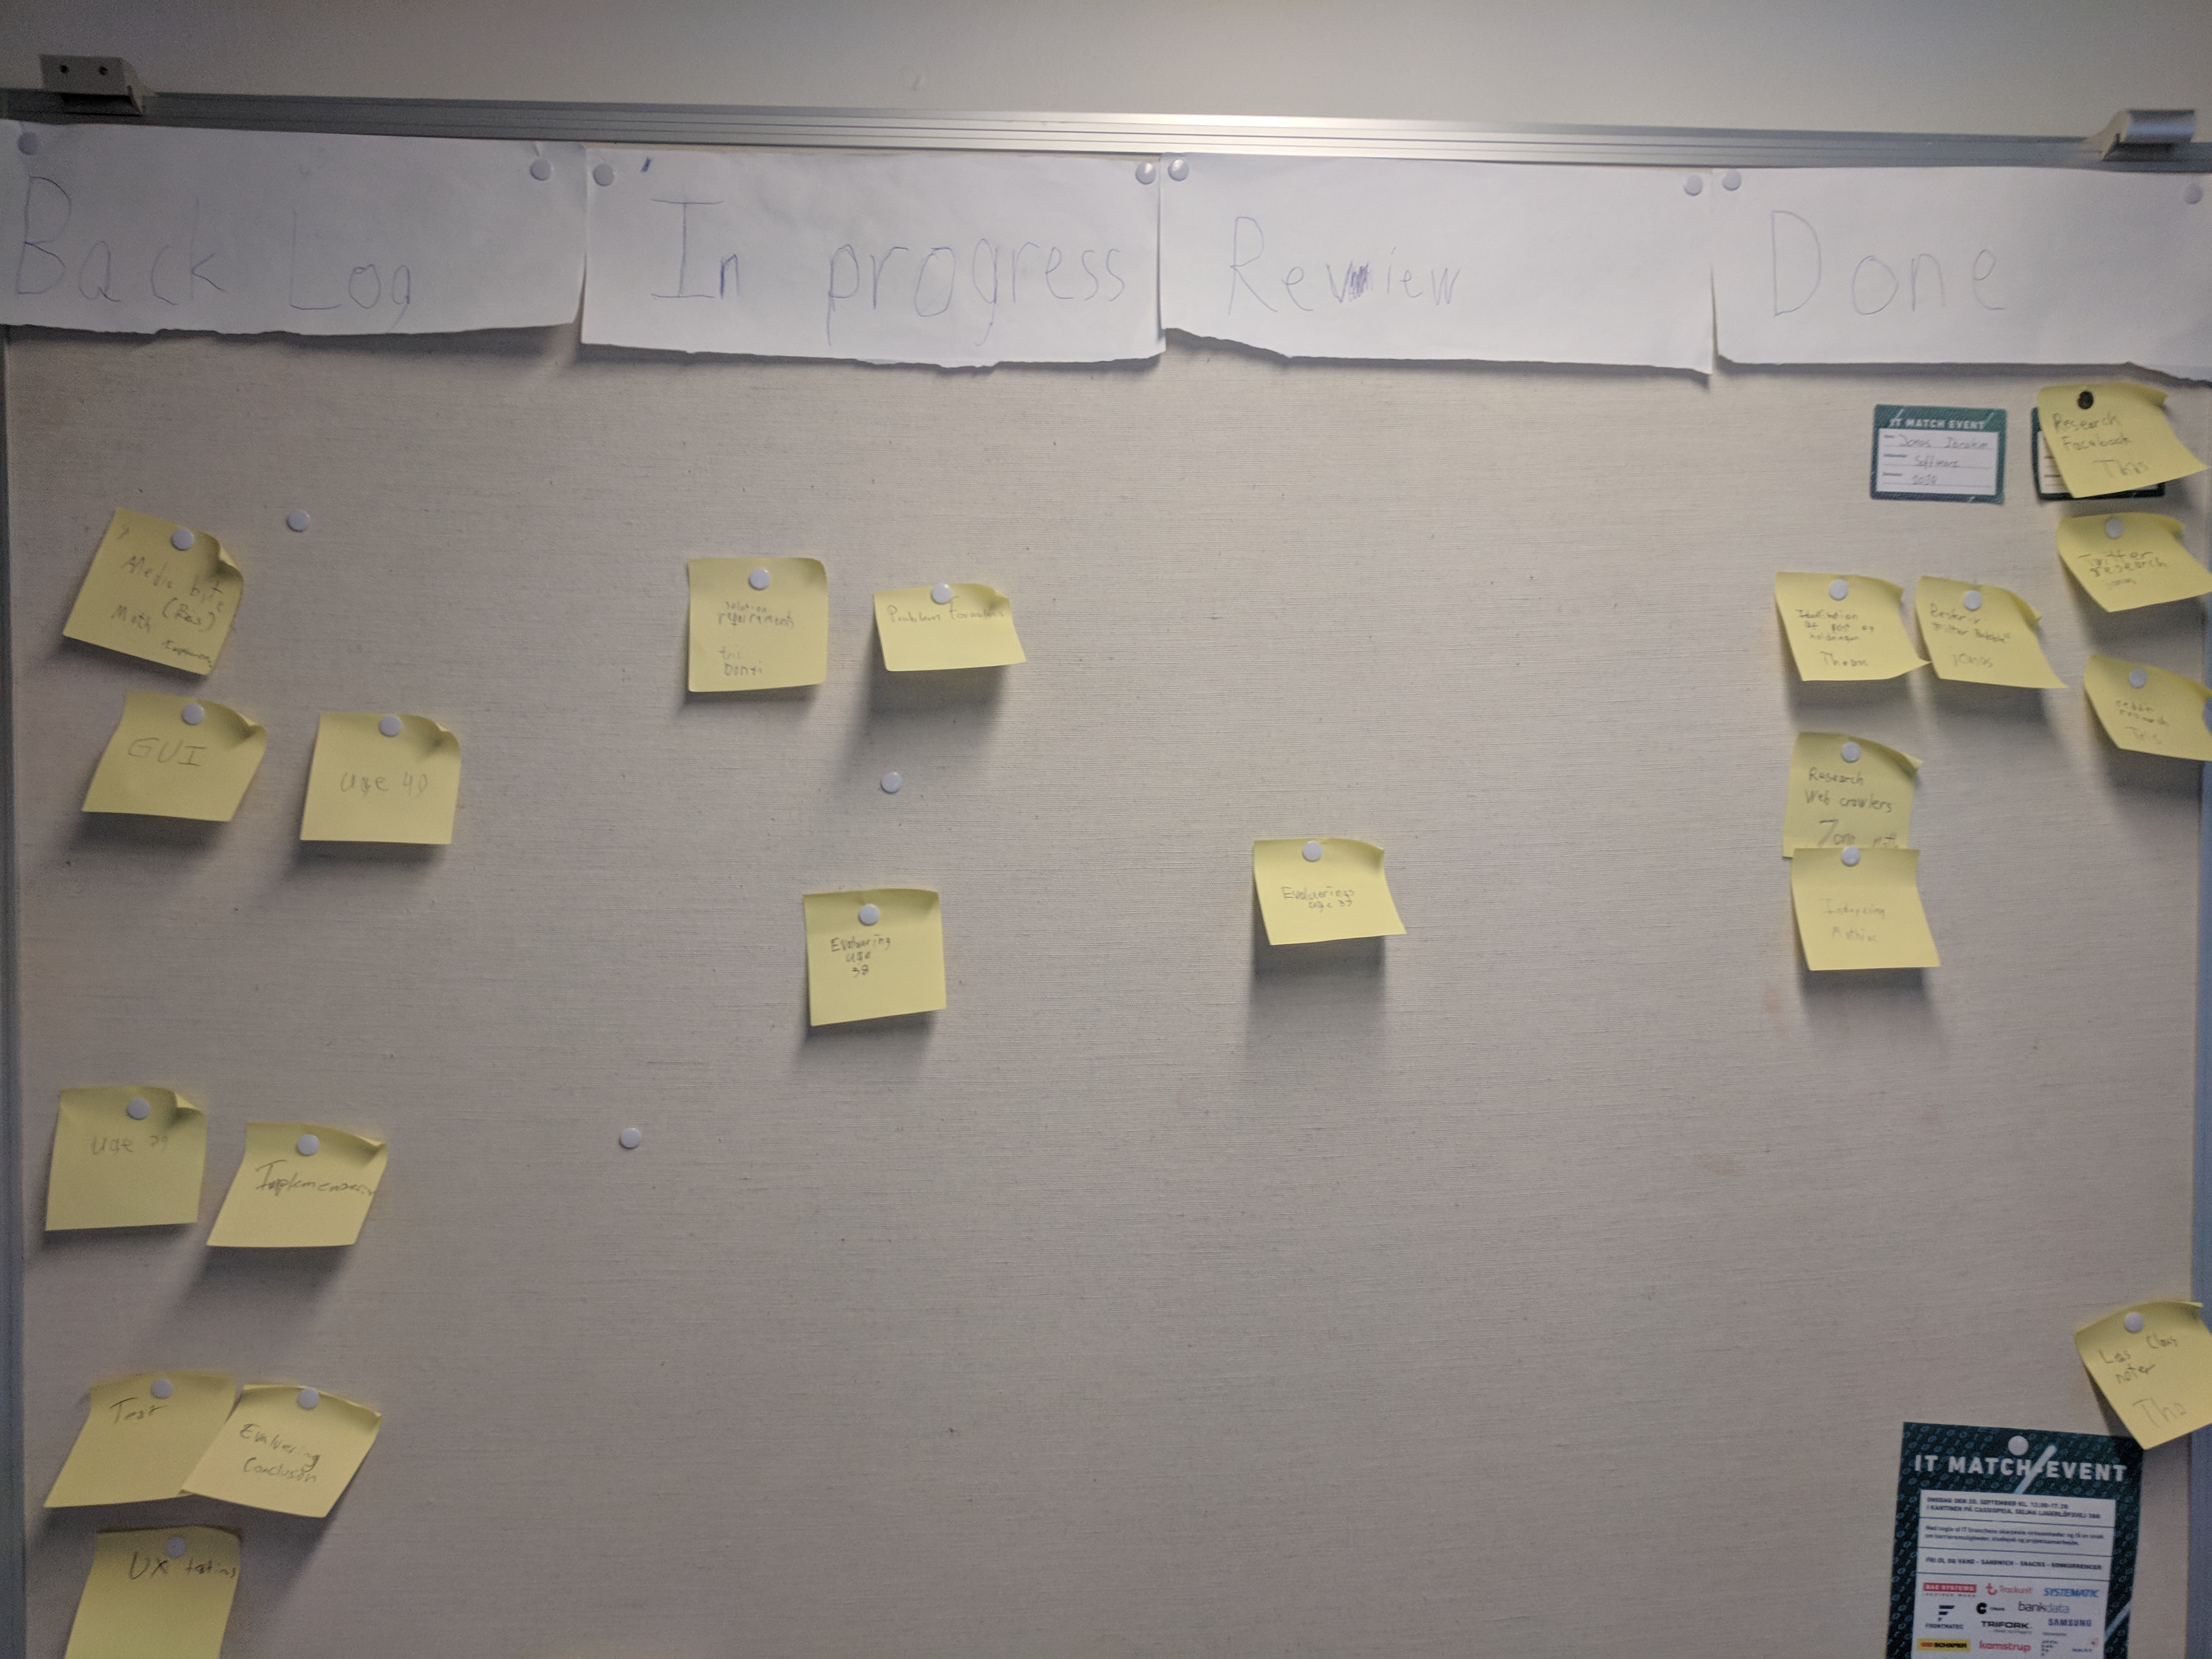
\includegraphics[width =
0.5\textwidth]{figures/Board.jpg}
	\caption{Our board SCRUM element.}
\end{figure}]

\subsection*{Reflection}
We had narrowed us down with the social media sites to the ones we thought were
best, therfore we investiated further and found many we had not considered. The
report is progressing but getting updates as we learn new stuff, perhaps we
should have studied some of the topics further to avoid much rewriting in the
analysis part. There are not many gaps in our schedule for project work this
semester, with all the lectures.

We have made some plans to improve the group's structure and workflow. We made a
short description of the final product, but it was mainly for the supervisor to
see, and it will definitely be updated after. We also look forward to seeing how
morning meetings will help with information sharing.

We found that Facebook is a very restrictive media, with its user-data, and does
not part with information easily. We would have to ask for permission to crawl
Facebook, and from the limited amount of crawlers permitted to do so, then it is
unlikely that we will get the chance. Therefore we are starting to look further into
Twitter and Reddit, as a source for user data, on the initial lookup Twitter's
data looks accessible.

\subsection*{Next Week}
During the next week we want to finish the parts of the report in editing, and
get the rest of the analysis into the editing phase. We would also like to get
started on the data gahtering part of the report. Nedxt week will have focus on
indexing the sites crawled, which means we hope that we are able to see the data
we will be working with.







% Facebook is restrictive, besides that we need to ask for permission. So far we
% are thinking of going in a different direction from facebook. We are looking
% into what is available with twitter and reddit. Alot seems to be available at
% twitter.
% 
% Klaus has had a dat 6 group. We have a degree so we can reach out to companies,
% and we seem more professional. We need a to reflect, and evaluate our UI. We can
% look into books and look for what design process we can follow to develop a UI.
% When we test it should not be a mock-up, but if nothing else provide the
% illusion of depth.
% 
% For reflection, we consider adding a chapter for describing the process.
% 
% We edited the filter bubble and Facebook research parts of the report and
% continued work on the webcrawler.
% Finished research on the links from Klaus, and structured an idea for the final
% webagent.
% Begun on the fundamental request builder to fetch information from Twitter.
% 
% 
% Mail Our Progress:
% We have found that Facebook does not seem to be that great for accurate data.
% We have researched on basic crawlers and its seems like we need permission to
% crawl.
% Twitter and Reddit seem like the best options from our current research.
% 
% The agenda for the meeting:
% 1. Web crawlers and limited access to major social hubs, Facebook doesn't want
% people to crawl their sites. While it seems to be limited on Twitter.
% 2. What do you expect from a 7th semester project? Aside from the semester
% description? 3. How should we document our process? Lone said we needed to
% describe this.
% 
% 
% 
% 
% Here are our notes from today's meeting 
% 
% ---------- Current idea
% for the structure of the rapport:
% Intro (problem description)
% 
% Research Social medial Data gathering Web agent?
% 
% Problem Formulation
% 
% GUI design
% 
% Implementation (done by 25. nov)
% 
% Test User tests Evaluation of the UI Other tests?
% 
% Evaluation
% 
% Rapport:
% Introduction seems good.
% Chapter 2 - Should be more distinctly separated, between formal and reflection.
% Be more concrete about everything, less would, should…
% 
% Discussion:
% Twitter has good possibilities, as we can access a lot of data through their
% API, though we can only make a limited amount of calls every 15 min.
% 
% Thoughts on UI:
% What should the user be shown? Can we find enough info to break the bubble We
% will need to briefly describe the process of designing a GUI but we do not need
% to describe the whole process of iterating through the designs.
% 
% Reflections:
% For the process we can describe some of the difficulties of having all the
% different combination of study. As we need to be better to manage our time. We
% should add our experiences with researching facebook, twitter and reddit and why
% we chose what we chose.

\section*{Week 39}
\subsection*{What Happend This Week}
We created an idea for the structure of the report, and what we wanted in the
chapters. We also set the date 25. November, as the day we would like to be done
with programming. The introduction part is finished, the other analysis chapter
needs to be more coherent.
We have also found that the Twitter \ac{API} gives us access to a vast amount of
user data, although they limit the number of calls we can make every 15 minutes, it
should not cause us any problems. We have made some considerations on the
\ac{UI} of our application. We are starting to consider how much user data we need to break
a filter bubble and if we can get from Twitter.
Our current idea for the semester goal: "We want to help an individual break out
of the filter bubble. The agent checks the user's web activity and provides
information from outside that bubble (how much and what is not finalized yet)."


\subsection*{Reflection}
It was a setback to find out how difficult it was to
get access to social media site's user data through a web crawler. We are now
investigating if there is a way to still use our crawler, we should definitely
have investigated further upon how we could use a crawler instead of its
development.
The Twitter \ac{API} does seem like a suitable option to gather enough user data
about a person, sources explaining that tweets can be used to break the bubble
have been found. Workflow is still a little slower than we liked, we think one
of the problems is that the group only have a full day of work on Mondays. We
learned that we need to be more direct and concise in our report and used too
loose terms such as many "could", "would" and "should".

\subsection*{Next Week}
In an attempt to get more done each week we will try
with a rule, stating that a member meets every day at 9:00 if there is no
lecture for that group member. Next week we want to finish the analysis part of
the report and be able to pull some data from Twitter with the Twitter \ac{API}.



% Our Progress:
%  We have had a busy schedule this week so we don't have much progress to show.
% However, we do have 2 chapters ready for you to read.
%  We have researched further on basic crawlers since it works well with one of
% our courses as well.
%    The agenda for the meeting:
%  1. Feedback on chapters.
%  2. We want to help an individual break out of the filter bubble. The agent
% checks the user's web activity and provides information from outside that
% bubble (how much and what is not finalized yet).

% Research Social medial Data gathering Web agent?  
% Problem Formulation 
% GUI design  
% Implementation (done by 25. nov)  Test User tests Evaluation of
% the UI Other tests?  Evaluation  Rapport:
% Introduction seems good.
% Chapter 2 - Should be more distinctly separated, between formal and
% reflection.
% Be more concrete about everything, less would, should…  Discussion:
% Twitter has good possibilities, as we can access a lot of data through their
% API, though we can only make a limited amount of calls every 15 min.
%  Thoughts on UI:
% What should the user be shown? Can we find enough info to break the bubble We
% will need to briefly describe the process of designing a GUI but we do not
% need to describe the whole process of iterating through the designs.
%  Reflections:
% For the process we can describe some of the difficulties of having all the
% different combination of study. As we need to be better to manage our time. We
% should add our experiences with researching facebook, twitter and reddit and
% why we chose what we chose.
%\section*{Week 40}
\subsection*{What Happend This Week}
This week we finished the initial problem and most of the analysis, which is
starting to be near a finishing point. We are now able to retrieve 3200 tweets
from each account a given user is following, meaning that if a user follows five
Twitter accounts then we will find 16000 assuming each account have 3200 tweets
or more.

We have spent some time thinking further upon how to use the vast amount of user
data, we are currently considering focusing on ``emotional wording'' such as
which hashtags and keywords go together, and if it is a positive or negative
tweet.

\subsection*{Reflection}
The application is progressing and we can gather user data now, however, we are
still working on improving the speed. We are not entirely sure about how to
handle the collected data, and we are still researching that. We are wondering
if we fulfil the requirements for the semester, and will discuss what we have
and expect to do and figure out if it is enough with our supervisor. It is
usually a requirement to bring along something from courses and which is
something we need to discuss as well. Our decision to meet at 9:00 is working,
and as a result, the project progress seems to be smoother.

\subsection*{Next Week} 
We will mainly perform edits and improve upon the code
next week because of a Programming Paradigms mini project. Therefore, we do not
expect much more progress.




% Mail
% Our Progress:
% Report: This week we have finished the following sections: Twitter Analysis,
% Initiating Problem and minor corrections (The acronyms in parentheses are marked
% because we haven’t added them properly yet).
% There are still sections in progress, not yet in the master.
% Code: We have managed to retrieve 3200 tweets for each account a given user is
% following. That is, if you follow "denmarkdotdk" and "VisitDenmark", we retrieve
% the 3200 most recent tweets from both of these accounts. We can store this data
% locally, and determine which words and hashtags in the tweets. Now we need to
% determine how we want to analyze the data, and the model we want to use to
% detect the "filter bubble". (We have mostly been talking about a neural network
% which attempts to classify the user's stance on a given subject by using words
% such as "stupid", "amazing", "idiot" etc.) Twitter seems like the best options
% from our current research.
% 
% The agenda for the meeting:
% - It's usually a requirement for us to bring something from our courses, how is
% it this semester? - Feedback

%  regarding the report: I only have minor comments, but rather a major comment
% outside the pdf: in the final report, there will be the scientific part and
% the reflection part (which is also scientific somehow .. ). However, it seems
% to me that in the report, there is also a sort of progress report included a
% bit, which won't be part of the final report. Let's talk about this tomorrow.
%  the code part: sounds exciting. Looking forward to hear more tomorrow.
%Worked on a GUI section (DEB terms), specifically we drew a storyboard and a sketch of the gui.

Reworked text and fixed grammatical errors. Reworked the title in analysis, began on problem statement, and finished working on most of the analysis.

Fixed the threads of the program
We are now able to find the average political value of a bias.

Scheme delivery
%\section*{Week 42}
\subsection*{What Happend This Week}
x

\subsection*{Evaluation}


\subsection*{Next Week}





% Our Progress:
% Report: We have restructured the research chapter of the report, and updated
% the problem formulation and it is ready for you to read. We have also
% formulated a list of requirements for our solution which we would like
% feedback on as well.
%  Code: Nothing noteworthy since the last update.
%  The agenda for the meeting:
% 1. Presentation 2. Feedback 3. Which approach would you recommend to analyse
% for the filter bubble data? So far, our data consists of friends, followers,
% tweets (words, hashtags, links, news media). We are unsure of how to best
% analyze this data.
% 4. Should we find live user test the solution with (would most likely be an
% American using Twitter)? 5. A requirement for the project is for our
% application to be internet-application, - agent, or -service. Since we use an
% API for all our Internet-related operations, would you consider this
% requirement as being met?

%\section*{Week 43}\label{Week43}
\subsection*{What Happend This Week}
On the report many corrections, some missing introductions and conclusions have
been fixed. From the meeting we found out that we wanted a \ac{GUI} web
application in Laravel \fix{ToDo}{Ref til Laravel} which should connect to a
queue server in C\# through a \ac{REST} \ac{API}. Then the queue should call a
modified version of our workers: program fetching tweets from Twitter. The
\ac{GUI} and workers communicate with a database through another \ac{REST}
\ac{API}. We split all members into different parts and progressed on all,
investigating how and what we should do with them. We quickly found that the
database \ac{REST} \ac{API} should be made in a separate Laravel project.

\subsection*{Evaluation}
During the presentation Monday we received a lot of feedback on everything, and
some keywords or methods extremely useful to us that we had not considered. Such
a presentation meeting is a very useful tool to strengthen a project and
something which should be done in future projects as well. New mini projects for
the complete project that we had not considered before were found through
brainstorming.

\subsection*{Next Week}
During the next week we will continue development on the parts, we have a lot to
do after this meeting. And we will make some considerations on which type of
user we want, university, high school or other? 
The web crawler chapter should be expanded with more information on the \ac{API}
and perhaps some information on why we describe the crawler since we will not
use it.


% All corrections on the report applied and a further grammar check on new
% stuff, introductions and conclusions are also added to the chapters.
%  After the meeting Monday, we discussed how to expand the program we have
% written to be a web application, as such we decided that we need a gui web
% application in Laravel which connects to a queue server in c# through a rest
% api, then the queue server should start workers which are a modified version
% of our first program. The gui and workers communicate with a database though
% another rest api. The rest of the week was spent on trying first to make the
% database rest api in c# but it was then after many problems it was decided
% that the database rest api should be made in a separate Laravel project. Each
% of the for a mentioned items has been worked on during the week.
%   ML-stuff In regards to classifying tweets the week has been spent
% investigating different types of ML, especially Support Vector Machines, Long
% Short Term Memory and basic Neural Networks, which have shown to be promising.
% There has been some thought regarding using different methods for sentiment
% analysis, such as bag of words vs NNs.
%  There has also been devoted time to figuring out whether we should write the
% ML part in python, as it has a lot of good libraries and documentation, or C#
% which has a what appears to be well regarded libraries and somewhat less
% documentation.
%  There has been work on figuring out how to transform tweets into something
% useful, and so far a tweet parser has been built, which transform the tweet
% from a string to a list of string (tokens).
% There has been thought about further transforming the list to a vector by
% mapping words with unique integers, which should be useful when used by a NN.
%  We have considered options for different methods of training, and arrived
% that we are going use the supervised method, though that means we will have to
% provide a lot of tweets which we will have to classify regarding political
% leaning.
%  Meeting:
% Presentation:
% Click on spectrum. Which friends are where.
% Tune what kind og people you want suggested. Very different, slightly
% different from you? Suggest people with a minimum of intellect (University
% degree? Known speaker?) Lookup existing recommendation systems. Current
% systems, reports, solutions? ADs API can maybe group people a bit? Maybe look
% at hashtags? What is our end goal? A plugin? Standalone application? Take
% additional input from the user. What do they think at the moment? What other
% information to supply? Accuracy can partly be determined by user feedback. Do
% you agree with our conclusion? Lookup study about what which hashtags imply
% about a political stance/leaning.
% Look at related work to ours.
% What is the complexity of our algorithm.
% Store information for lookup later.
% Have two approaches system based/neural network. How do they compare? If we
% want to do preprocessing/plugin/(neural network?) we can ask for access to
% (something? computer??)  Meeting:
% Problem with information about reddit user numbers.
% We could "potentially" just write about why our application would be easy to
% scale, and how we would do it  Should we find people to test the application?
% - Maybe, if we can.
%  How do we expand our application:
% - How would we deal with increased popularity - We should probably do
% something with a browser (plugin/site/server/etc.)  What to do:
% - User interface (Laravel) - Describe Architecture MVC front-end. Unknown on
% back-end - Algorithm which uses emotional words, keywords, and hashtags - If
% people log in using their own account, they get an amount of requests for
% themselves - Convert system to run on a server - Definitely do something to
% consider scalability e.g. multiple servers, or using users own requests -
% Begin writing reflections (what should we have done? What did we do? The
% plan?) - Plan how to systematically evaluate our application. User interface,
% testers, usability, functionality (does it work as intended).
% - Look at lecture notes on how to design interfaces. Then do what the slides
% tell us to do.
% - Expand the webcrawler chapter with more info on the different parts of it,
% and in the end a conclusion with the reasonings why we won’t use it (and
% causes like spoofing and a very naughty crawler) - Lookup existing
% recommendation systems. Current systems, reports, solutions?

%\section*{Week 44}
\subsection*{What Happend This Week}
We made an early model of a solution including some machine intelligence and
wrote about sentiment analysis. We set-up the database and the \ac{API} for the
database and the authorization for the \ac{API} for the database, and an
implementation part for it in the report Queue server and \ac{REST} \ac{API} for
queues server Setup \ac{GUI} using Laravel and started working on Twitter
authentication.

\subsection*{Evaluation}
We are happy with the direction it is going now, but the workload feels much
harder than before the meeting last week. However, we feel like we are on the
right track, and we talked with our supervisor about getting another meeting
with the expert on a later date. The machine intelligence part seems to be
difficult, and we are running into some problems. Therefore, a person will be
assigned to create an algorithm in case it does not work out as intended.

\subsection*{Next Week} 
Next week we hope to have a better idea about how to classify tweets, and
keep up with progress being made.

% We made an early model of our neural network and wrote about sentiment
% analysis.
%  We setup the database and the API for the database and the authorazation for
% the API for the database, and an implementation part for it in the report 
% Queue server and REST API for queues server  Setup GUI using Laravel and
% started working on twitter authentication  and documentation in the report
% were started for the semester

%The week Nov5-10 in progress
%\section*{Week 46} \subsection*{What Happend This Week} 
A feature which retrieves tweets from a set of pre-classified political point of
view (left/right) users, and determines what words they are more likely to use.
This requires a large amount of users with pre-known alignments. To begin, we
have manually compiled a list of Twitter users, which the queue server \ac{API}
now interacts with. The queue server is able to queue jobs for execution. The
queue server instance uses the worker for each job. The worker has been adapted
for use by different threads, such that the limits are not the same for each
thread. We have classified 120 tweets by hand, into 5 classes: Right, little
right, neutral, little left, left.


\subsection*{Reflection} 
We should have started earlier on these weekly summaries and made our notes
better from the beginning, it has caused some mixup and issues doing the clean
writing of them in the report. We have tried to get the same kind of result from
the Naïve Bayes model and algorithm to classify the tweets, this is good since
it permits us to use both or find the one which works best.


\subsection*{Next Week} 
Next week will be slow because of a mini project in Programming Paradigms. Else
everyone has something to work on which will likely not be finished doing that
week.



% We would like feedback on the two weekly summaries, we would like to know if
% the format is fitting.
%   Status:
% We have added a feature to the program which retrieves tweets from a set of
% pre-classified (left/right) users, and determine what words they are more
% likely to use. The idea behind this is, that if we can identify what words are
% most likely to be used by users of specific political alignments, we can
% dynamically update our list of keywords, which we already use for classifying
% users. This, however, requires a large amount of users with pre-known
% alignments. To begin, we have manually compiled a list of twitter users, which
% we use to get started with the word gathering. The idea is, that whenever we
% classify a user with a high degree of certainty, we can add that user to our
% list of users from which we identify words. We have also begun commenting the
% code.
%  The queue server api now interacts with the queue server instance and are
% able to queue jobs for execution. The queue server instance uses the worker
% for each job. The worker has been adapted for use by different threads, such
% that the limits are not the same for each thread.
% Then work began on the section for the queue server api.
%  Did more research into dense feature vectors and other solutions. Found an
% algorithm called word2vec that is interesting.
% With 120 tweets which we have classified by hand, into 5 classes: Right,
% little right, neutral, little left, left. With these tweets we trained a Naive
% Bayesian with bad results, with 5 classes it had a 26% success rate, with 3
% classes it had 44% success. Used a simple SVM with a 3 classes, it had a
% success rate of 30%.
%  Added a TextProcessing Library to the project, which allows us to process
% tweets.
%   As for the agenda:
% We would like feedback on the weekly summaries from the report
